% !TeX program = xelatex
\documentclass[10pt,a4paper]{article}
\usepackage[margin=20mm,top=18mm,bottom=20mm]{geometry}
\usepackage{fontspec}
\setmainfont{texgyretermes-regular.otf}[BoldFont=texgyretermes-bold.otf,ItalicFont=texgyretermes-italic.otf,BoldItalicFont=texgyretermes-bolditalic.otf]
\setsansfont{texgyreheros-regular.otf}[BoldFont=texgyreheros-bold.otf,ItalicFont=texgyreheros-italic.otf,BoldItalicFont=texgyreheros-bolditalic.otf]
\usepackage{amsmath,amssymb,graphicx,booktabs,array,longtable,tabularx}
\usepackage{microtype,xcolor,caption,titlesec,enumitem}
\usepackage[numbers,sort&compress]{natbib}
\usepackage{xurl}
\usepackage[hidelinks,unicode]{hyperref}
\definecolor{CloudraInk}{HTML}{173B2A}
\captionsetup{font=small,labelfont=bf,labelsep=period,skip=5pt}
\titleformat{\section}{\large\bfseries}{\thesection}{0.5em}{}
\titleformat{\subsection}{\normalsize\bfseries}{\thesubsection}{0.5em}{}
\titleformat{\subsubsection}{\normalsize\bfseries}{\thesubsubsection}{0.5em}{}
\titlespacing*{\section}{0pt}{2ex plus .5ex minus .3ex}{.8ex}
\titlespacing*{\subsection}{0pt}{1.6ex plus .4ex minus .3ex}{.7ex}
\setlength{\parindent}{1em}
\setlength{\parskip}{2pt}
\setlength{\emergencystretch}{1.5em}
\setlength{\textfloatsep}{10pt plus 3pt minus 2pt}
\setlength{\floatsep}{9pt plus 2pt minus 2pt}
\setlength{\LTpre}{7pt}
\setlength{\LTpost}{7pt}
\renewcommand{\topfraction}{.9}
\renewcommand{\bottomfraction}{.85}
\renewcommand{\textfraction}{.08}
\renewcommand{\floatpagefraction}{.7}
\renewcommand{\thesection}{S\arabic{section}}
\renewcommand{\thefigure}{S\arabic{figure}}
\renewcommand{\thetable}{S\arabic{table}}
\renewcommand{\theequation}{S\arabic{equation}}
\renewcommand{\thepage}{S\arabic{page}}
\renewcommand{\bibfont}{\small}
\setlength{\bibsep}{3pt plus 1pt}
\setcounter{tocdepth}{2}
\makeatletter
\renewcommand*\l@subsection{\@dottedtocline{2}{1.5em}{3.2em}}
\makeatother
\raggedbottom
\begin{document}
\begin{center}
{\LARGE\bfseries Supplementary Information\par}
\vspace{0.6em}
{\large\bfseries Cloudra: Geometric Reasoning and Scientific Validation for Autonomous Reaction Mechanism Exploration\par}
\vspace{0.6em}
{\normalsize Chengyi Yang\,\textsuperscript{1}, Qianxin Zhou\,\textsuperscript{2,†}, and Yang Li\,\textsuperscript{1,†}\par}
\vspace{0.4em}
{\small \textsuperscript{1}College of Chemistry and Pharmaceutical Engineering, Changsha University of Science and Technology, Changsha 410114, China\par
\textsuperscript{2}State Key Laboratory of Photocatalysis on Energy and Environment, College of Chemistry, Fuzhou University, Fuzhou 350002, China\par}
\vspace{0.3em}
{\footnotesize \textsuperscript{†}Qianxin Zhou and Yang Li contributed equally as co-second authors.\par}

\vspace{0.6em}
{\small Draft --- 31 October 2026\par}
\end{center}
\noindent This supplement provides the experimental protocol, layered evaluation, complete task and score tables, expanded diagnostic analyses, literature source register, and machine-readable materials accompanying the manuscript. Standard denotes the same-model backbone comparison; Record and Brief are workflow ablations. Section, table, figure, equation, and page numbers carry the prefix S to distinguish them from the main text.
\tableofcontents
\section{Benchmark design and experimental protocol}
\label{sec:si-protocol}

\subsection{Task specification and study units}
CloudraBench comprises 50 tasks, distributed as 20 Easy, 10 Normal, 10 Hard, and 10 Impossible tasks. Easy tasks cover elementary transformations, conformational changes, and basic execution; Normal tasks require intermediate identification and continuity across elementary steps; Hard tasks emphasize competing pathways and stereochemical identity; Impossible tasks require conclusions appropriate to the capabilities of the allowed electronic-structure methods. A task fixes the reactant and target identities, reaction conditions, total charge, spin multiplicity, requested deliverables, and permitted methods. These specifications are common to the workflow configurations compared on that task. The complete task catalogue accompanies the per-task results.

The repeated-task study is identified as P1b and the full-benchmark study as P2. Two studies provide complementary experimental units (Table~\ref{tab:si-study-design}). The repeated-task study contains three independent runs for each combination of four tasks and four configurations. E1 concerns elimination preorganization; NB1 concerns multistep decarboxylation; HA1 concerns stereochemical ring opening; and IA1 concerns an electronic-structure method limitation. The full-benchmark study contains one retained run for each of the 50 tasks under each configuration. Its primary matched unit is therefore a task represented in all four configurations. The 48 repeated-task runs and the 200 full-benchmark runs are reported as separate studies.

\begin{table}[htbp]
\centering
\caption{Experimental units in the two studies.}
\label{tab:si-study-design}
\small
\begin{tabular}{p{0.21\textwidth}p{0.31\textwidth}p{0.34\textwidth}}
\toprule
Design & Repeated-task study (P1b) & Full-benchmark study (P2) \\
\midrule
Task set & E1, NB1, HA1, IA1 & All 50 CloudraBench tasks \\
Backbone & DeepSeek-v4.1-flash (1017) & DeepSeek-v4.1-flash (1017); official DeepSeek chat-completions API \\
Configurations & Guided, Standard, Record, Brief-errors & Guided, Standard, Record, Brief-errors \\
Repetitions & Three per task and configuration & One retained run per task and configuration \\
Task-level runs & $4\times4\times3=48$ & $50\times4=200$ \\
Elapsed-time unit & Four-task batch at concurrency two; three batches per configuration & Computational effort on the common 15-task subset \\
\bottomrule
\end{tabular}
\end{table}

\subsection{Workflow configurations and primary comparison}
Guided is compared primarily with the actual Standard branch using the same model backbone. Record and Brief-errors isolate changes to scientific acceptance and diagnostic presentation within the available workflow (Table~\ref{tab:si-configurations}). Standard retains access to computational tools while hiding explicit delivery-DAG tools, removing scientific acceptance interception, and providing neutral computational feedback. Guided retains the delivery graph, scientific checks, and detailed diagnostics. Record retains available tools and recording while removing mandatory scientific acceptance. Brief-errors retains guidance and acceptance while shortening diagnostics. The task and method restrictions are not relaxed in an ablation.

\begin{table}[htbp]
\centering
\caption{Operational definition of the four workflow configurations. Brief-errors is abbreviated as Brief in figures and tables; Standard is also labelled Backbone.}
\label{tab:si-configurations}
\small
\begin{tabular}{p{0.16\textwidth}p{0.25\textwidth}p{0.25\textwidth}p{0.22\textwidth}}
\toprule
Configuration & Delivery-graph interface & Mandatory scientific acceptance & Diagnostic presentation \\
\midrule
Guided & Explicit & Retained & Detailed \\
Standard & Explicit DAG tools hidden & Removed & Neutral computation feedback \\
Record & Available tools and records retained & Removed & Recording retained \\
Brief-errors & Retained & Retained & Shortened \\
\bottomrule
\end{tabular}
\end{table}

Both studies used DeepSeek-v4.1-flash (1017). The API alias is \texttt{deepseek-v4-flash} in all eight frozen coordinator and follower configurations and in their actual model-call telemetry.\citep{deepseekv42026} Model names, campaign identifiers, budgets, stopping reasons, and artifacts are retained with the corresponding runs. Cloudra revision 70daa5a identifies the implementation described in the main-text methods.\citep{ref14} This implementation identifier, the experiment records, and the scoring and organization records serve different purposes: software or API versions are taken from the applicable archive rather than inferred from a later installed environment or model alias.

\subsection{P2 model configuration and campaign versions}
\label{sec:si-p2-model-metadata}

P1b denotes the repeated-task study: four tasks, four workflow configurations, and three runs per combination, giving 48 task runs. P2 denotes the full-benchmark study of 50 tasks under the four configurations, giving 200 retained task runs. The P2b and P2c execution campaigns supply this P2 dataset. Three completed P2b runs were retained (Guided/D3, Record/D1, and Standard/D3), and P2c supplied the remaining 197 runs.

The deployed backbone was DeepSeek-v4.1-flash (1017), as specified by the authors. All eight P2 configuration snapshots, one for each campaign and workflow combination, specify \texttt{deepseek-v4-flash} for both the coordinator and follower slots. The request-start and completion telemetry in all eight runtime archives records the same model identifier. Cloudra called the official DeepSeek endpoint through streaming OpenAI-compatible chat completions. The frozen \texttt{native\_search=auto} setting selects this route in the campaign-era implementation. Table~\ref{tab:si-p2-model-metadata} records the request settings and execution versions. The deployment name and version are reported alongside the literal API alias preserved in the execution records.

\begin{table}[htbp]
\centering
\small
\caption{Frozen P2 configuration and campaign metadata. Request settings describe the harness configuration; telemetry counts are provided in the accompanying \texttt{p2\_model\_metadata.json}.}
\label{tab:si-p2-model-metadata}
\begin{tabular}{p{0.27\linewidth}p{0.66\linewidth}}
\toprule
Item & Recorded value \\
\midrule
Deployed model & DeepSeek-v4.1-flash (1017) \\
Provider and API alias & DeepSeek; \texttt{deepseek-v4-flash} in all eight snapshots and their request/completion telemetry \\
Endpoint and transport & \url{https://api.deepseek.com}; streaming chat completions \\
Role slots & Coordinator and follower use the same provider, model identifier, and request settings \\
Reasoning setting & Requested \texttt{reasoning\_effort=minimal} \\
Temperature & 1.0 in the archived run-start settings \\
Context window & 400,000 tokens in the frozen harness configuration \\
Spawned-agent budget & \texttt{max\_tokens=32768} in the archived \texttt{agent.spawned} settings; this is the per-agent request setting, not the run's total token consumption \\
Tool invocation & JavaScript protocol \\
Retained task runs & Three from P2b and 197 from P2c \\
Task concurrency & Two per configuration, eight in total \\
Campaign starts & P2b: 25 October 2026, 18:01:17 UTC+8; P2c: 25 October 2026, 22:18:45 UTC+8 \\
Campaign base & \texttt{53309d0e} \\
Configuration commits & Guided: \texttt{6e89d20c}; Record: \texttt{746c33f0}; Standard: \texttt{c7fc94a1}; Brief-errors: \texttt{3b9831bb}. Both campaigns use these commits. \\
\bottomrule
\end{tabular}
\end{table}

The configuration commits identify experiment execution. The implementation reference used to describe the system, subsequent evaluator fixes, and publication-table reproduction have their own version records. The companion metadata file gives archive-relative source members for each configuration and runtime record. Its request-start and completion counts refer to the archived runtime events, including auxiliary LLM activity and cancelled P2b attempts; the benchmark sample remains the 200 retained task runs.

\paragraph{Fixed geometric heuristics.}
The atom-map ranking uses fixed coefficients: 2 for each formed or broken bond, 1 for each bond-order change, 4 for a hydrogen-count mismatch, 8 for charge or radical-electron mismatches, and 2 for a stereochemical mismatch. The $J_{\min}+2$ window retains near-optimal maps when reporting ambiguity. The branch-crowding descriptor also uses fixed implementation heuristics: decay $\rho=0.5$, traversal through depth five, and a congestion flag when the four-branch total $B_{\mathrm{axis}}\geq9.0$. These settings rank or annotate candidate structures. Quantum-chemical evidence determines their subsequent physical qualification. The imaginary-mode participation ratio has a comparison value of 0.5; its alignment flag is advisory, and strict acceptance uses the first-order-saddle and IRC/endpoint evidence.

\paragraph{Conformational sampling.}
The default preorganization uses topology-aware rigid placements and guided MMFF94 relaxation, followed by energy/RMSD selection. Its standard multicomponent settings sample 32 relative orientations and retain up to eight guided placements. The separate conformer-search tool defaults to the RDKit backend and also provides an external CREST backend\citep{crest2020} for additional conformer or noncovalent-complex sampling. The default CREST route uses GFN2-xTB with the quick setting. Search outputs enter the calculation workflow as candidate geometries and undergo the task-specific stationary-point and pathway checks.



\subsection{Allowed calculations and reference definitions}
Easy, Normal, and Hard tasks permit xTB, PM7, and B3LYP-D3(BJ)/def2-SVP.\citep{gfn2xtb2019,pm72013,becke1993,lyp1988,stephens1994,d32010,d3bj2011,def22005} Impossible tasks are restricted to xTB and PM7. Native ORCA, Gaussian, and MOPAC records supply the corresponding computational quantities and termination information.\citep{orca2025,gaussian16,mopac2026,ref11} Each result is associated with the engine, calculation level, species, and task conditions represented in its source record.

The reference answer (Gold) specifies the mechanistic species and elementary steps, stereochemical identities, applicable numerical targets, and explicit negative targets. Numerical activation barriers use electronic energies at a consistent level of theory:
\begin{equation}
\Delta E_e^{\ddagger}=E_{\mathrm{TS},e}-E_{\mathrm{ref},e}.
\label{eq:si-barrier}
\end{equation}
These benchmark barriers do not include zero-point or thermal corrections. The energy reference is the verified stable minimum of the corresponding species. Declared conformational connections within the same species can share that stable reference; a conformational conversion itself retains its own starting conformer as the reference. Distinct stereochemical substrates and independent channel contact complexes retain separate references. The actual IRC connection and the energy denominator are recorded separately, so a stable reference is not automatically identified with the conformer reached directly by an IRC.

Reference treatment follows the individual task definition. NB1\_E2 and NQ5\_E2 have no numerical reference under the specified proton-transfer policy. IB9 combines a numerical first-step reference of 5.65~kcal~mol$^{-1}$ with a negative second-step target. The qualitative selectivity tasks and numerical tolerance settings are specified in Section~\ref{sec:si-scoring}. Reference status belongs to the corresponding reference record; task availability, presence of a Gold graph, and physical acceptance of a complete reference chain are recorded separately.

\subsection{Physical evidence associated with a mechanism}
A delivered mechanism represents species occurrences as nodes and elementary steps as edges. A species minimum requires convergence and a frequency calculation with zero imaginary frequencies. An accessible transition-state step requires a first-order saddle with exactly one imaginary frequency associated with the intended reaction, together with direction evidence linking that saddle to the declared endpoint species.\citep{ref09,ref10} Native normal termination, geometry convergence, frequencies, and pathway connectivity are checked as separate facts.

The direction evidence starts at the same transition state in the two IRC directions. The actual outer frame from each direction is connected through a converged optimization to an endpoint minimum with zero imaginary frequencies and the appropriate chemical identity and stereochemistry. The IRC trajectory itself need not converge all the way to either minimum when this outer-frame--optimization--frequency chain establishes the connection. The archived frames and their calculation lineage are retained. Geometric interval measurements assist interpretation; they do not replace a supported native endpoint chain. For separated products, the required constituent minima are verified; an intact molecular complex is evaluated as the corresponding whole-system species.

These requirements apply to the objects requested by the task. An explicitly negative target is represented as inaccessible with its basis retained. A species-only negative question does not require an invented transition state, process edge, or numerical barrier.

\subsection{Offline organization and publication records}
Formal evaluation is conducted after the run artifacts are organized into the common mechanism-graph representation. Organization uses that run's conversations, tool records, reports, geometries, and native calculation outputs to recover graph objects, repair file references, and convert quantities already present in the run. Human organization and field-level sources are recorded, and the same organizational rules apply across configurations. The resulting graph expresses the scientific content of the run; Gold is used for evaluation rather than as a source of additional run conclusions or computational evidence.

The full-benchmark publication table contains 200 runs and all 600 Graph, Self-consistency, and Accuracy component values. Each published composite is aligned with its own existing component records. The 200 released composite scores are retained; the weighted components reproduce them to their four-decimal reporting precision. The publication tables separately preserve whether the run itself generated a root mechanism graph and whether the graph was subsequently organized offline. Thus, the original delivery behavior and the organized scientific score remain separately inspectable quantities.

The repeated-task study retains its historical four-configuration snapshots. The subsequent Standard offline organization is a separately identified update to those records; it is not labelled as a new uniform rescore of all 48 runs. Analyses using the repeated-task archive specify which record supplies the result.

\subsection{Paired statistical analysis and time measurements}
For a task $i$ and configuration $a$, let $S_{ia}$ denote its composite score. Configuration means give each task equal weight within the reported set. The primary paired difference is
\begin{equation}
\overline{\Delta}_{\mathrm{G-S}}=\frac{1}{n}\sum_{i=1}^{n}
\left(S_{i,\mathrm{Guided}}-S_{i,\mathrm{Standard}}\right).
\label{eq:si-paired-difference}
\end{equation}
The same calculation is used within each tier and for the combined Normal/Hard subset. Weighted component contributions are the mean paired component differences multiplied by 0.1, 0.3, and 0.6, respectively. They add to the composite difference up to the reporting precision of the released scores.

The 95\% percentile intervals use 100,000 task-cluster bootstrap samples with seed 20261031. Each resampled task carries its four configuration records together, preserving the paired comparison. The bootstrap unit is a task, not an elementary edge or an individual quantum-chemical calculation.

The repeated-task elapsed-time analysis uses the recorded start and finish of each four-task batch at concurrency two: three batches per configuration, or 12 batches in total. Its unit is batch wall-clock hours. The full-benchmark effort analysis uses the 15 tasks with common effort records across all four configurations, comprising 60 task-level runs. It reports calculation counts and cumulative quantum-chemical job-hours, obtained by summing the individual calculation durations within a run. In the archived Standard/M1 extraction, native-log CPU time is divided by four to obtain the corresponding job-duration estimate. Job-hours are neither core-hours nor a measurement of the full P2 research-run wall-clock duration. These time quantities retain their distinct denominators and units throughout the supplementary tables.

\section{Layered scoring and scientific completion}
\label{sec:si-scoring}

\subsection{Composite and reporting layers}
For a formally organized run, the reported composite combines graph structure $G$, physical self-consistency $C$, and accuracy $A$:
\begin{equation}
S=0.1G+0.3C+0.6A.
\label{eq:si-composite}
\end{equation}
The three components are retained separately. Execution status, original graph delivery, completion of requested steps, graded physical evidence, and complete scientific acceptance are also reported separately. A completed process or a partial score does not substitute for the evidence required by a particular scientific claim.

\subsection{Graph structure and chemical correspondence}
The graph component measures coverage of the reference mechanism by the delivered mechanism. Transition-state nodes are folded into their elementary-step edges for graph comparison. Species are matched chemically and reaction steps are compared through their endpoints and atom-mapped bond changes. RDKit supplies chemical representations and NetworkX supplies graph representation and matching.\citep{ref13,networkx2008} Missing reference elements, incorrect chemical identities, or mismatched accessibility declarations contribute edit costs. Additional delivered nodes or edges are not penalized merely for being additional in this component.

The tier-specific graph comparison ignores stereochemistry for Easy and Normal tasks and retains it for Hard tasks. Bound native evidence determines the evidence association of a delivered species. The graph score is not multiplied by the binary self-consistency pass flag: graph coverage and physical self-consistency remain distinct components.

\subsection{Graded physical self-consistency}
The self-consistency assessment operates on delivered species and steps, independently of numerical agreement with Gold. A transition-state step receives graded credit for the evidence stages in Table~\ref{tab:si-self-consistency}. A complete verified chain receives 1.0. When necessary, evaluation searches the same run's native artifacts for the corresponding chain; recovery of a file association retains the same physical acceptance criteria.

\begin{table}[htbp]
\centering
\caption{Graded self-consistency contribution for an accessible transition-state step. The endpoint contribution is 0.25 for one verified side and 0.50 for both sides.}
\label{tab:si-self-consistency}
\small
\begin{tabular}{p{0.65\textwidth}r}
\toprule
Evidence stage & Contribution \\
\midrule
Verified first-order saddle: exactly one imaginary frequency & 0.35 \\
IRC starting geometry consistent with the selected saddle & 0.15 \\
Native outer-frame--optimization--frequency lineage to both declared endpoint minima & 0.50 \\
\bottomrule
\end{tabular}
\end{table}

For graphs containing reaction edges, $C$ is the mean of the delivered edge scores. An edge without a transition-state node requires both endpoint species to be covered. For a species-only graph, $C$ is the mean species-coverage score. Explicit inaccessible targets are exempt from requirements for physically nonexistent stationary points or paths and receive the corresponding self-consistency credit.

The complete self-consistency pass is a separate all-required-elements condition. It checks the required species and steps, including minimum evidence and the full transition-state/IRC chain. Consequently, a full graded component and a binary scientific-acceptance record are retained as separate outputs. Counts of $C=1$ in the main text and supplementary score tables refer to full component scores; they are not renamed as counts of fully accepted complete mechanisms. Fractional scores identify the attained stages of physical support.

\subsection{Electronic barriers and numerical accuracy}
For a numerical reference step, the declared barrier is checked against an energy difference derived from its native calculation evidence. An omitted edge barrier can be obtained from the delivered transition-state and starting-species energies when those quantities and their native records support the conversion. The energy difference is converted from hartree to kcal~mol$^{-1}$ using the common conversion factor 627.509474.

For a supported numerical value $\widehat{\Delta E}_e^{\ddagger}$ and reference $\Delta E_{e,\mathrm{Gold}}^{\ddagger}$, the underlying Gaussian score is
\begin{equation}
q_e=\exp\left[-\frac{\left(\widehat{\Delta E}_e^{\ddagger}-
\Delta E_{e,\mathrm{Gold}}^{\ddagger}\right)^2}{2\sigma_e^2}\right].
\label{eq:si-gaussian}
\end{equation}
The released task rubrics use base widths of 3.0~kcal~mol$^{-1}$ for Easy and Impossible tasks and 2.0~kcal~mol$^{-1}$ for Normal and Hard tasks. For a reference barrier at or below 10.0~kcal~mol$^{-1}$, the reference-comparison width is the larger of the base width and 5.0~kcal~mol$^{-1}$. This small-barrier width applies to comparison with Gold; the declaration-to-log consistency check retains the task's base width.

All reference edges remain in the accuracy denominator, with their recorded weights. A numerical reference edge lacking a matching delivered step, a declared barrier, or a log-derived value receives zero for that edge. Other evidenced steps retain their contributions. Numerical deviations on supported reference edges are aggregated with a maximum penalty fraction of 0.3; missing-step/evidence penalties and incorrect negative conclusions are not protected by this numerical-deviation cap. More explicitly, for total reference-edge weight $W$, supported numerically graded edges $D$, and missing or incorrectly delivered targets $U$, the aggregation takes the form
\begin{equation}
A=1-\min\!\left(\frac{\sum_{e\in D}w_e(1-q_e)}{W},\,0.3\right)
-\frac{\sum_{e\in U}w_e}{W}.
\label{eq:si-accuracy-aggregation}
\end{equation}
Correct negative targets and accessible edges intentionally lacking a numerical reference contribute their prescribed full-credit terms through $W$. The latter are not interpreted as numerical barrier predictions.

The evaluator considers the legal transition-state/reference-energy combinations present in the delivered evidence. When those records contain a combination agreeing with Gold but the reported value uses a different supported conformer or energy-reference definition, the documented answer-definition treatment assigns an edge score of 0.9 in place of $q_e$. A declared barrier that is unsupported by any legal evidence combination, with no reference-consistent alternative in the delivered records, triggers the integrity short circuit: the composite retains only $0.1G$, and the self-consistency and accuracy contributions are zeroed. An omitted step is handled by its missing contribution rather than by this inconsistent-declaration rule.

\subsection{Qualitative selectivity and property targets}
HA1, HA6, HB1, and HF1 use a qualitative favored-channel target in the accuracy slot. The delivered mechanism must identify one favored edge corresponding to the reference channel or its chemically matched product. Product identity supplies the chemical correspondence when the delivered channel label differs from the internal reference label. The numerical channel spread is not scored as a quantitative selectivity prediction in these tasks. HL1 instead retains its independently referenced channel barriers and does not use this favored-channel substitution.

When a task specifies species properties, its accuracy assessment compares the declared properties with the corresponding reference targets. Numerical property widths are 0.02~\AA\ for bond lengths, 50~cm$^{-1}$ for frequency quantities, and 2.0~kcal~mol$^{-1}$ for energy differences; the specific keyed property determines the width. Specified state-ordering text is compared after case and whitespace normalization. Multiple specified properties contribute their mean score.

\subsection{Impossible tasks and final scientific claims}
Impossible-task assessment is based on the final delivered target. Correctly identifying that a requested target is inaccessible or outside the allowed method's capability earns the corresponding negative-target credit. An exploratory calculation followed by a correct negative conclusion is not penalized for having been attempted. An incorrect positive accessibility claim, a purportedly trustworthy barrier/property value for the negative target, or an absent required negative conclusion loses the corresponding credit. Negative endpoint species are treated consistently with their associated negative step. A species-only negative target is assessed without introducing a process edge.

The result must be interpreted at the identity of the requested target. A valid result for another electronic state, species, or pathway does not automatically answer the stated question. The per-task tables and case analyses retain this target association alongside the numerical score.

\subsection{Original delivery, organized evaluation, and score reproduction}
Original delivery completeness records whether the run generated its mechanism graph during execution. Organized evaluation records the graph obtained by the formal offline procedure in Section~\ref{sec:si-protocol}. The publication component table preserves each run's original or organized score record and field provenance; existing released scores are reproduced rather than replaced by scores from a later software environment.

The retained reproduction procedure joins the released run table to the corresponding recorded components and reconstructs the aggregate tables and figure data. Its checks cover 200 unique task/configuration records, 600 nonmissing component values, and consistency of the weighted components with the 200 released totals. The maximum absolute difference from the published four-decimal composites is $4.9711\times10^{-5}$. The scoring formulas above explain the layered evaluation; regenerating publication tables requires the retained component records, while independently reassessing native scientific evidence additionally uses the associated run artifacts and evaluator revision.

\section{CloudraBench task catalogue}
\label{sec:task-catalogue}

CloudraBench comprises 20 Easy, 10 Normal, 10 Hard, and 10 Impossible tasks. Tables~\ref{tab:catalogue-easy}--\ref{tab:catalogue-impossible} list the chemical task, charge and multiplicity, stated conditions, and task-specific research target. The task names and molecular inputs are retained in the accompanying machine-readable catalogue; the original task definitions additionally specify atom mappings, complete prompts, reference graphs, and scoring settings.

Method set A comprises xTB, PM7, and B3LYP-D3(BJ)/def2-SVP and applies to Easy, Normal, and Hard tasks. Method set B comprises xTB and PM7 and applies to Impossible tasks. The research target is evaluated within its assigned method set. Reaction-mechanism tasks request a graph of the investigated species and elementary steps, electronic activation barriers for the steps actually computed, and bound stationary-point and pathway evidence. Stereochemical tasks additionally require identities established from the computed geometries. The rows below state the distinguishing target for each task rather than restating this shared delivery protocol.

For Impossible tasks, the listed quantity or process remains the question posed to the agent. The task evaluates the final conclusion under the allowed methods: an appropriately supported negative conclusion is a valid deliverable, and exploratory calculations need not be presented as trustworthy target properties. Species-property questions do not acquire invented process edges or transition states.

\begingroup
\small
\setlength{\tabcolsep}{3.5pt}
\renewcommand{\arraystretch}{1.15}
\begin{longtable}{@{}p{0.065\linewidth}p{0.285\linewidth}p{0.60\linewidth}@{}}
\caption{Easy-tier task catalogue. Method set A applies to every task in this table.}\label{tab:catalogue-easy}\\
\toprule
ID & Chemical task & Stated conditions and task-specific research target \\
\midrule
\endfirsthead
\multicolumn{3}{l}{\tablename\ \thetable\ (continued)}\\
\toprule
ID & Chemical task & Stated conditions and task-specific research target \\
\midrule
\endhead
\midrule
\multicolumn{3}{r}{Continued on the next page}\\
\endfoot
\bottomrule
\endlastfoot
D1 & butadiene + ethylene Diels-Alder (parent DA)\newline {\footnotesize Charge 0; multiplicity 1.} & \textit{Conditions:} gas phase, 487--648 \({}^{\circ}\mathrm{C}\) kinetics.\newline \textit{Target:} Cycloaddition pathway, stationary points, and electronic activation barrier. \\
\addlinespace[3pt]
D3 & cyclopentadiene dimerization (self Diels-Alder)\newline {\footnotesize Charge 0; multiplicity 1.} & \textit{Conditions:} gas/liquid phase, slow at room temperature.\newline \textit{Target:} Dimerization pathway, stationary points, and electronic activation barrier. \\
\addlinespace[3pt]
D4 & cyclopentadiene + acrolein Diels-Alder\newline {\footnotesize Charge 0; multiplicity 1.} & \textit{Conditions:} gas phase or hydrocarbon solvent, heated.\newline \textit{Target:} Cycloaddition pathway, stationary points, and electronic activation barrier. \\
\addlinespace[3pt]
E1 & F- + CH3CH2Cl elimination -> ethylene + HF + Cl-\newline {\footnotesize Charge -1; multiplicity 1.} & \textit{Conditions:} gas phase.\newline \textit{Target:} Elimination pathway from the pre-reaction complex, stationary points, and electronic activation barrier. \\
\addlinespace[3pt]
F1 & BH4- + formaldehyde -> borane-methoxide adduct [CH3OBH3]-\newline {\footnotesize Charge -1; multiplicity 1.} & \textit{Conditions:} gas phase.\newline \textit{Target:} Hydride-transfer pathway to the borane--methoxide adduct, stationary points, and electronic barrier. \\
\addlinespace[3pt]
F4 & BH3 + formaldehyde -> methoxyborane via Lewis adduct\newline {\footnotesize Charge 0; multiplicity 1.} & \textit{Conditions:} gas phase.\newline \textit{Target:} Lewis-adduct-mediated conversion to methoxyborane, with the investigated species and elementary steps. \\
\addlinespace[3pt]
G2 & diimide cis reduction of ethylene\newline {\footnotesize Charge 0; multiplicity 1.} & \textit{Conditions:} gas phase.\newline \textit{Target:} Reduction pathway, stationary points, and electronic activation barrier. \\
\addlinespace[3pt]
G3 & propylene + ethylene ene reaction (Alder-ene)\newline {\footnotesize Charge 0; multiplicity 1.} & \textit{Conditions:} gas phase, high temperature.\newline \textit{Target:} Ene-reaction pathway, stationary points, and electronic activation barrier. \\
\addlinespace[3pt]
L1 & cyclobutene -> butadiene ring opening\newline {\footnotesize Charge 0; multiplicity 1.} & \textit{Conditions:} gas phase, 403-448 K.\newline \textit{Target:} Ring-opening pathway, stationary points, and electronic activation barrier. \\
\addlinespace[3pt]
L2 & hexatriene -> cyclohexadiene ring closure\newline {\footnotesize Charge 0; multiplicity 1.} & \textit{Conditions:} gas phase, 390-434 K.\newline \textit{Target:} Electrocyclic ring-closure pathway, stationary points, and electronic activation barrier. \\
\addlinespace[3pt]
M1 & 2,2'-dimethylbiphenyl aryl-aryl rotation\newline {\footnotesize Charge 0; multiplicity 1.} & \textit{Conditions:} gas phase.\newline \textit{Target:} Aryl--aryl rotational pathway, connected conformers, and rotational barrier. \\
\addlinespace[3pt]
M14 & acrolein s-trans <-> s-cis rotation\newline {\footnotesize Charge 0; multiplicity 1.} & \textit{Conditions:} gas phase.\newline \textit{Target:} s-trans/s-cis conformers, their connecting pathway, and rotational barrier. \\
\addlinespace[3pt]
M15 & HONO cis-trans isomerization\newline {\footnotesize Charge 0; multiplicity 1.} & \textit{Conditions:} gas phase.\newline \textit{Target:} cis/trans structures, their connecting pathway, and isomerization barrier. \\
\addlinespace[3pt]
M16 & formic acid dehydrogenation HCOOH -> CO2 + H2\newline {\footnotesize Charge 0; multiplicity 1.} & \textit{Conditions:} gas phase.\newline \textit{Target:} Dehydrogenation pathway and electronic activation barrier. \\
\addlinespace[3pt]
M17 & methyl isocyanide -> acetonitrile rearrangement\newline {\footnotesize Charge 0; multiplicity 1.} & \textit{Conditions:} gas phase.\newline \textit{Target:} Isomerization pathway to acetonitrile and electronic activation barrier. \\
\addlinespace[3pt]
M3 & NH3 umbrella inversion\newline {\footnotesize Charge 0; multiplicity 1.} & \textit{Conditions:} gas phase.\newline \textit{Target:} Inversion pathway, stationary points, and inversion barrier. \\
\addlinespace[3pt]
M8 & cyclohexane chair flip\newline {\footnotesize Charge 0; multiplicity 1.} & \textit{Conditions:} gas phase.\newline \textit{Target:} Chair-interconversion pathway, relevant conformers, and barrier. \\
\addlinespace[3pt]
P2 & cyclopentadiene degenerate H shift\newline {\footnotesize Charge 0; multiplicity 1.} & \textit{Conditions:} gas phase or solution, fast at room temperature.\newline \textit{Target:} Degenerate hydrogen-shift pathway, stationary points, and electronic activation barrier. \\
\addlinespace[3pt]
P3 & allyl vinyl ether Claisen rearrangement\newline {\footnotesize Charge 0; multiplicity 1.} & \textit{Conditions:} gas phase, \(\sim\)200 \({}^{\circ}\mathrm{C}\).\newline \textit{Target:} Claisen-rearrangement pathway, stationary points, and electronic activation barrier. \\
\addlinespace[3pt]
X1 & beta-propiolactone -> ethylene + CO2\newline {\footnotesize Charge 0; multiplicity 1.} & \textit{Conditions:} gas phase, \(\sim\)350 \({}^{\circ}\mathrm{C}\).\newline \textit{Target:} Decomposition pathway to ethylene and carbon dioxide, with stationary points and barrier. \\
\addlinespace[3pt]
\end{longtable}
\endgroup

\begingroup
\small
\setlength{\tabcolsep}{3.5pt}
\renewcommand{\arraystretch}{1.15}
\begin{longtable}{@{}p{0.065\linewidth}p{0.285\linewidth}p{0.60\linewidth}@{}}
\caption{Normal-tier task catalogue. Method set A applies to every task in this table.}\label{tab:catalogue-normal}\\
\toprule
ID & Chemical task & Stated conditions and task-specific research target \\
\midrule
\endfirsthead
\multicolumn{3}{l}{\tablename\ \thetable\ (continued)}\\
\toprule
ID & Chemical task & Stated conditions and task-specific research target \\
\midrule
\endhead
\midrule
\multicolumn{3}{r}{Continued on the next page}\\
\endfoot
\bottomrule
\endlastfoot
NB1 & malonic acid thermal decarboxylation: malonic acid -> acetic acid + CO2\newline {\footnotesize Charge 0; multiplicity 1.} & \textit{Conditions:} gas-phase thermolysis.\newline \textit{Target:} Identify intermediates and preserve elementary-step continuity through decarboxylation to the final products. \\
\addlinespace[3pt]
NI1 & imine formation: formaldehyde + methylamine -> N-methylmethanimine + water\newline {\footnotesize Charge 0; multiplicity 1.} & \textit{Conditions:} gas phase; optimal around pH 4-6 (bell-shaped rate profile).\newline \textit{Target:} Identify the addition/condensation intermediates and connecting elementary steps leading to the imine and water. \\
\addlinespace[3pt]
NI5 & imine formation (aqueous): formaldehyde + methylamine -> N-methylmethanimine + water\newline {\footnotesize Charge 0; multiplicity 1.} & \textit{Conditions:} aqueous solution, weakly acidic (pH 4-6, bell-shaped rate profile).\newline \textit{Target:} Resolve the aqueous imine-formation network and relevant proton-transfer steps under the stated conditions. \\
\addlinespace[3pt]
NQ1 & aromatic Claisen rearrangement: allyl phenyl ether -> 2-allylphenol\newline {\footnotesize Charge 0; multiplicity 1.} & \textit{Conditions:} gas phase; thermal, \(\sim\)200 \({}^{\circ}\mathrm{C}\).\newline \textit{Target:} Resolve rearrangement and subsequent conversion to 2-allylphenol, retaining the intermediate network. \\
\addlinespace[3pt]
NQ5 & oxy-Cope rearrangement: 1,5-hexadien-3-ol -> hex-5-enal ([3,3] then enol-keto tautomerization)\newline {\footnotesize Charge 0; multiplicity 1.} & \textit{Conditions:} gas phase, heated.\newline \textit{Target:} Resolve the [3,3] rearrangement and enol--keto tautomerization as the investigated network. \\
\addlinespace[3pt]
NR1 & formamide dehydration: formamide -> hydrogen cyanide + water\newline {\footnotesize Charge 0; multiplicity 1.} & \textit{Conditions:} Gas phase; isolated neutral, closed-shell formamide; no added water, acid, or catalyst.\newline \textit{Target:} Investigate formimidic-acid intermediates and conformational transitions in the neutral dehydration network. \\
\addlinespace[3pt]
NU3 & H3P=CH2 ylide + formaldehyde -> ethylene + H3P=O\newline {\footnotesize Charge 0; multiplicity 1.} & \textit{Conditions:} salt-free model conditions (gas-phase ylide, closest to model chemistry).\newline \textit{Target:} Resolve the salt-free model Wittig-reaction network to ethylene and phosphine oxide. \\
\addlinespace[3pt]
NU5 & Passerini reaction: formaldehyde + formic acid + methyl isocyanide -> N-methyl-alpha-formyloxyacetamide\newline {\footnotesize Charge 0; multiplicity 1.} & \textit{Conditions:} dichloromethane (DCM), room temperature, high concentration.\newline \textit{Target:} Resolve the three-component Passerini-reaction network to the specified alpha-acyloxy amide. \\
\addlinespace[3pt]
NU6 & Staudinger beta-lactam synthesis: ketene + methanimine -> 2-azetidinone\newline {\footnotesize Charge 0; multiplicity 1.} & \textit{Conditions:} ketene generated in situ; inert solvent.\newline \textit{Target:} Identify the ketene--imine addition and beta-lactam-forming network, retaining any identified intermediate. \\
\addlinespace[3pt]
NY3 & isocyanic acid hydrolysis: HNCO + one water -> ammonia + carbon dioxide\newline {\footnotesize Charge 0; multiplicity 1.} & \textit{Conditions:} Gas phase; neutral closed-shell system with exactly one water molecule; no added solvent, acid, counterion, or catalyst.\newline \textit{Target:} Investigate carbamic-acid intermediates and connecting conformers without presupposing a fixed number of steps. \\
\addlinespace[3pt]
\end{longtable}
\endgroup

\begingroup
\small
\setlength{\tabcolsep}{3.5pt}
\renewcommand{\arraystretch}{1.15}
\begin{longtable}{@{}p{0.065\linewidth}p{0.285\linewidth}p{0.60\linewidth}@{}}
\caption{Hard-tier task catalogue. Method set A applies to every task in this table.}\label{tab:catalogue-hard}\\
\toprule
ID & Chemical task & Stated conditions and task-specific research target \\
\midrule
\endfirsthead
\multicolumn{3}{l}{\tablename\ \thetable\ (continued)}\\
\toprule
ID & Chemical task & Stated conditions and task-specific research target \\
\midrule
\endhead
\midrule
\multicolumn{3}{r}{Continued on the next page}\\
\endfoot
\bottomrule
\endlastfoot
HA1 & 3-methylcyclobutene ring opening: determine the stereochemical outcome\newline {\footnotesize Charge 0; multiplicity 1.} & \textit{Conditions:} gas phase or inert solvent, \(\sim\)150--200 \({}^{\circ}\mathrm{C}\), thermal.\newline \textit{Target:} Determine stereochemical products and channel identities; report channel barriers and the requested relative preference. \\
\addlinespace[3pt]
HA6 & trans-3,4-dimethylcyclobutene ring opening: determine the stereochemical outcome\newline {\footnotesize Charge 0; multiplicity 1.} & \textit{Conditions:} gas phase or inert solvent, heating, thermal.\newline \textit{Target:} Determine stereochemical products and channel identities; report channel barriers and the requested relative preference. \\
\addlinespace[3pt]
HA8 & (2E,4Z,6E)-octa-2,4,6-triene thermal 6-pi electrocyclization: determine the stereochemical outcome\newline {\footnotesize Charge 0; multiplicity 1.} & \textit{Conditions:} Gas phase; first thermal ground-state electrocyclization only; no subsequent hydrogen shifts or photochemistry.\newline \textit{Target:} Resolve the product stereochemistry of the first thermal electrocyclization; report investigated channel identities and barriers. \\
\addlinespace[3pt]
HB1 & cyclopentadiene + maleic anhydride Diels-Alder: determine endo/exo outcome\newline {\footnotesize Charge 0; multiplicity 1.} & \textit{Conditions:} benzene, room temperature or mild heating.\newline \textit{Target:} Determine endo/exo products, channel barriers, and relative preference. \\
\addlinespace[3pt]
HB10 & cyclopentadiene + acrylonitrile Diels-Alder reaction: determine both stereochemical pathways\newline {\footnotesize Charge 0; multiplicity 1.} & \textit{Conditions:} Gas phase; concerted addition; common reactant-complex reference for the two channels.\newline \textit{Target:} Compute both endo/exo pathways using a common reactant-complex reference; report identities and barriers. \\
\addlinespace[3pt]
HD2 & cyclohexene oxide + hydroxide: determine the stereochemical outcome of the epoxide opening\newline {\footnotesize Charge -1; multiplicity 1.} & \textit{Conditions:} aqueous NaOH, heat.\newline \textit{Target:} Determine the stereochemistry of the epoxide-opening product from the computed structures. \\
\addlinespace[3pt]
HF1 & cyclohex-2-en-1-ol peracid epoxidation: determine the stereochemical outcome\newline {\footnotesize Charge 0; multiplicity 1.} & \textit{Conditions:} performic acid, CH2Cl2, 0--25 \({}^{\circ}\mathrm{C}\).\newline \textit{Target:} Determine the two facial pathways, product stereochemistry, barriers, and relative preference. \\
\addlinespace[3pt]
HH1 & 1,1'-binaphthyl thermal racemization\newline {\footnotesize Charge 0; multiplicity 1.} & \textit{Conditions:} thermal racemization, \(\sim\)50 \({}^{\circ}\mathrm{C}\), DMF.\newline \textit{Target:} Characterize the thermal racemization pathway, stereochemical endpoints, and barrier. \\
\addlinespace[3pt]
HI1 & Cope elimination of threo/erythro N,N-dimethyl-3-phenyl-2-butylamine oxide: determine the stereochemical mapping\newline {\footnotesize Charge 0; multiplicity 1.} & \textit{Conditions:} Gas phase; isolated neutral singlet amine oxide. Treat threo and erythro substrates as two separate systems and retain explicit stereochemical SMILES.\newline \textit{Target:} Compute threo and erythro substrates separately; establish substrate CIP assignments and alkene E/Z identity from 3D geometries. Use each substrate's own minimum for its barrier. \\
\addlinespace[3pt]
HL1 & formonitrile oxide + norbornene [3+2] cycloaddition: determine both facial pathways\newline {\footnotesize Charge 0; multiplicity 1.} & \textit{Conditions:} Gas phase; neutral singlet formonitrile oxide and unsubstituted norbornene. Compare approach from both faces relative to the methano bridge.\newline \textit{Target:} Compute both facial approaches relative to the methano bridge and assign products from 3D geometries. Use each channel's own stable contact minimum; report contact-conformer energies separately. \\
\addlinespace[3pt]
\end{longtable}
\endgroup

\begingroup
\small
\setlength{\tabcolsep}{3.5pt}
\renewcommand{\arraystretch}{1.15}
\begin{longtable}{@{}p{0.065\linewidth}p{0.285\linewidth}p{0.60\linewidth}@{}}
\caption{Impossible-tier task catalogue. Method set B applies to every task in this table.}\label{tab:catalogue-impossible}\\
\toprule
ID & Chemical task & Stated conditions and task-specific research target \\
\midrule
\endfirsthead
\multicolumn{3}{l}{\tablename\ \thetable\ (continued)}\\
\toprule
ID & Chemical task & Stated conditions and task-specific research target \\
\midrule
\endhead
\midrule
\multicolumn{3}{r}{Continued on the next page}\\
\endfoot
\bottomrule
\endlastfoot
IA1 & cyclobutadiene D4h automerization\newline {\footnotesize Charge 0; multiplicity 1.} & \textit{Conditions:} gas phase, low temperature (matrix isolation regime).\newline \textit{Target:} Thermal automerization of rectangular cyclobutadiene through the square transition structure: mechanism and activation barrier. \\
\addlinespace[3pt]
IA5 & cyclobutene disrotatory ring opening\newline {\footnotesize Charge 0; multiplicity 1.} & \textit{Conditions:} gas phase, thermal.\newline \textit{Target:} Thermal disrotatory ring opening of cyclobutene to butadiene: mechanism and activation barrier. \\
\addlinespace[3pt]
IA7 & Bergman cyclization of (Z)-hex-3-ene-1,5-diyne\newline {\footnotesize Charge 0; multiplicity 1.} & \textit{Conditions:} gas phase, thermal.\newline \textit{Target:} Bergman cyclization to p-benzyne: mechanism and activation barrier. \\
\addlinespace[3pt]
IA9 & 1,2-dioxetane thermolysis to two formaldehyde\newline {\footnotesize Charge 0; multiplicity 1.} & \textit{Conditions:} gas phase, thermal.\newline \textit{Target:} Thermolysis of 1,2-dioxetane to two formaldehyde molecules: mechanism and activation barrier. \\
\addlinespace[3pt]
IB9 & diazomethane and ethylene to cyclopropane via 1-pyrazoline\newline {\footnotesize Charge 0; multiplicity 1.} & \textit{Conditions:} gas-phase thermolysis.\newline \textit{Target:} Conversion of diazomethane and ethylene to cyclopropane and nitrogen through 1-pyrazoline. \\
\addlinespace[3pt]
IC3 & phenylnitrene open-shell singlet state\newline {\footnotesize Charge 0; multiplicity 3.} & \textit{Conditions:} gas phase.\newline \textit{Target:} Singlet--triplet energy gap and the electronic character of the lowest phenylnitrene singlet state. \\
\addlinespace[3pt]
ID2 & anomalous bonding in dioxygen difluoride (FOOF)\newline {\footnotesize Charge 0; multiplicity 1.} & \textit{Conditions:} gas phase, low temperature.\newline \textit{Target:} Equilibrium F--O and O--O distances of FOOF and its F--O bond-dissociation energy. \\
\addlinespace[3pt]
IE2 & nitrogen triple-bond dissociation curve\newline {\footnotesize Charge 0; multiplicity 1.} & \textit{Conditions:} gas phase.\newline \textit{Target:} Ground-state N2 dissociation curve and bond-dissociation energy. \\
\addlinespace[3pt]
IF3 & triangulene triplet ground state and singlet-triplet gap\newline {\footnotesize Charge 0; multiplicity 3.} & \textit{Conditions:} gas phase (surface-synthesis analogue).\newline \textit{Target:} Ground-state spin multiplicity and singlet--triplet gap of triangulene. \\
\addlinespace[3pt]
IG8 & chromium dimer ground-state dissociation curve\newline {\footnotesize Charge 0; multiplicity 1.} & \textit{Conditions:} gas phase.\newline \textit{Target:} Ground-state Cr2 potential-energy curve and bond-dissociation energy. \\
\addlinespace[3pt]
\end{longtable}
\endgroup


\section{Detailed benchmark results and scientific attribution}
\label{sec:si-detailed-results}

\subsection{Complete workflow and tier comparisons}

The publication dataset contains 200 task runs: one retained run for each of 50 tasks under Guided, Standard, Record, and Brief. Each run has a composite score and all three component scores. Table~\ref{tab:si-arm-tier} reports the means without pooling away the task tiers. Standard is the actual comparison branch using the same model backbone. Record and Brief vary the workflow's persistent acceptance requirements and diagnostic feedback, respectively.

\begin{table}[!htbp]
\centering
\small
\caption{Composite and component means for each workflow and task tier.}
\label{tab:si-arm-tier}
\begin{tabular}{llrrrrr}
\toprule
Tier & Workflow & $n$ & Composite & Graph & SC & Accuracy \\
\midrule
All & Guided & 50 & 0.7803 & 0.8788 & 0.9233 & 0.6924 \\
 & Standard & 50 & 0.5940 & 0.7837 & 0.5303 & 0.5943 \\
 & Record & 50 & 0.7044 & 0.7876 & 0.7177 & 0.6839 \\
 & Brief & 50 & 0.7415 & 0.8430 & 0.8468 & 0.6720 \\
\addlinespace
Easy & Guided & 20 & 0.8809 & 0.9620 & 0.9250 & 0.8454 \\
 & Standard & 20 & 0.7305 & 0.9007 & 0.5858 & 0.7744 \\
 & Record & 20 & 0.9443 & 0.9576 & 0.9050 & 0.9618 \\
 & Brief & 20 & 0.9054 & 0.9523 & 0.9125 & 0.8940 \\
\addlinespace
Normal & Guided & 10 & 0.7370 & 0.8589 & 0.9021 & 0.6342 \\
 & Standard & 10 & 0.5731 & 0.7607 & 0.5217 & 0.5675 \\
 & Record & 10 & 0.5287 & 0.6786 & 0.5783 & 0.4789 \\
 & Brief & 10 & 0.5857 & 0.7472 & 0.7740 & 0.4646 \\
\addlinespace
Hard & Guided & 10 & 0.9577 & 0.9107 & 0.9542 & 0.9672 \\
 & Standard & 10 & 0.6887 & 0.8481 & 0.5033 & 0.7549 \\
 & Record & 10 & 0.8723 & 0.9243 & 0.6650 & 0.9672 \\
 & Brief & 10 & 0.8282 & 0.9286 & 0.7767 & 0.8372 \\
\addlinespace
Impossible & Guided & 10 & 0.4451 & 0.7006 & 0.9100 & 0.1700 \\
 & Standard & 10 & 0.2473 & 0.5083 & 0.4550 & 0.1000 \\
 & Record & 10 & 0.2325 & 0.4200 & 0.5350 & 0.0500 \\
 & Brief & 10 & 0.4829 & 0.6345 & 0.8583 & 0.2700 \\
\bottomrule
\end{tabular}
\par\smallskip\begin{minipage}{\linewidth}\footnotesize SC denotes the graded self-consistency component. Every mean is calculated from the complete publication table. The overall tier weights are 20/50 for Easy and 10/50 for each other tier.\end{minipage}
\end{table}


Table~\ref{tab:si-pairwise} gives all six pairwise comparisons on the same 50 tasks. Guided--Standard has a mean difference of 0.186302, a median difference of 0.107950, and 35 task wins, eight losses, and seven ties. The 95\% task-bootstrap interval is [0.100268, 0.275854]. Within the Normal tier, the means are 0.737020 and 0.573050, with a difference of 0.163970 [0.036520, 0.292230] and seven wins in ten tasks. Within Hard, the means are 0.957650 and 0.688750; the difference is 0.268900 [0.121300, 0.445930], with Guided higher in all ten task pairs. Easy has means of 0.880940 and 0.730485, with 11 wins, five losses, and four ties; its paired median difference is 0.020850. Impossible has means of 0.445060 and 0.247330 and is examined at the level of the requested target below.

\begin{table}[!htbp]
\centering
\small
\caption{All pairwise composite-score comparisons across the 50 tasks.}
\label{tab:si-pairwise}
\begin{tabular}{lrrr}
\toprule
Comparison & Mean difference & 95\% interval & W/L/T \\
\midrule
Guided--Record & +0.0759 & [+0.0121, +0.1438] & 27/8/15 \\
Guided--Standard & +0.1863 & [+0.1003, +0.2759] & 35/8/7 \\
Guided--Brief & +0.0388 & [-0.0317, +0.1076] & 26/10/14 \\
Record--Standard & +0.1104 & [+0.0167, +0.2062] & 28/13/9 \\
Record--Brief & -0.0371 & [-0.0999, +0.0258] & 15/23/12 \\
Standard--Brief & -0.1475 & [-0.2474, -0.0494] & 12/33/5 \\
\bottomrule
\end{tabular}
\par\smallskip\begin{minipage}{\linewidth}\footnotesize The difference is the first workflow minus the second. W/L/T gives the first workflow's task wins, losses, and ties. Percentile task-bootstrap intervals use 100,000 resamples and seed 20261031; the four configurations of each sampled task remain together.\end{minipage}
\end{table}


The component decomposition in Table~\ref{tab:si-weighted-gain} expresses each contribution in composite-score units. Across all tasks, the self-consistency contribution is +0.117875 and the accuracy contribution +0.058916. In Normal and Hard together, the composite difference is +0.216435, including +0.124688 from self-consistency and +0.083712 from accuracy. Hard's accuracy contribution, +0.127391, accompanies a +0.135250 self-consistency contribution. These quantities describe the requested comparative study at two levels: the answer reached and the evidence supporting its attribution.

\begin{table}[!htbp]
\centering
\small
\caption{Weighted decomposition of the Guided--Standard composite difference.}
\label{tab:si-weighted-gain}
\begin{tabular}{lrrrrr}
\toprule
Scope & $n$ & Composite & $0.1\Delta G$ & $0.3\Delta SC$ & $0.6\Delta A$ \\
\midrule
All & 50 & +0.186302 & +0.009513 & +0.117875 & +0.058916 \\
Easy & 20 & +0.150455 & +0.006130 & +0.101750 & +0.042579 \\
Normal & 10 & +0.163970 & +0.009823 & +0.114125 & +0.040033 \\
Hard & 10 & +0.268900 & +0.006259 & +0.135250 & +0.127391 \\
Impossible & 10 & +0.197730 & +0.019226 & +0.136500 & +0.042000 \\
Normal + Hard & 20 & +0.216435 & +0.008041 & +0.124688 & +0.083712 \\
\bottomrule
\end{tabular}
\par\smallskip\begin{minipage}{\linewidth}\footnotesize Component contributions are calculated from the recorded unrounded components. Composite differences retain released composite scores, so the final displayed digits can differ by score rounding.\end{minipage}
\end{table}


The ablations give additional resolution. Guided--Record averages +0.075892 [0.012134, 0.143818] across all tasks. In Normal and Hard together, its +0.146845 composite difference decomposes into +0.008338 from graph, +0.091938 from self-consistency, and +0.046574 from accuracy. Guided--Brief averages +0.038816 [$-0.031704$, 0.107648], with mean differences of +0.151350 on Normal and +0.129470 on Hard. The task-level records retain both the general patterns and the crossed outcomes: NB1 has composite scores of 0.9628, 0.9128, and 0.9900 for Guided, Standard, and Brief; Guided and Brief both have self-consistency 1. NI1 has Guided and Standard composites of 0.9958 and 0.6196, with self-consistency 1 and 0.35. NQ5 favors Record over Guided, while NU3 favors Brief. Multistep performance is therefore resolved through the individual pathways and their evidence relationships.

\subsection{Runtime delivery and the organized scientific record}

During execution, Guided, Record, and Brief each produced 50 root mechanism graphs. Standard produced 43. Its remaining seven studies---F1, HA1, HF1, IA9, M17, NR1, and P3---were organized offline from their own conversations, reports, tool results, and calculation artifacts. The resulting analysis contains 50 organized graphs per workflow and 200 complete score profiles. Offline organization follows the evaluation procedure described in the methods and retains the source of each recovered field.

The seven Standard studies have a mean organized composite of 0.153743, compared with 0.828529 for Guided on the same tasks. Their contribution is 50.7\% of the total Guided--Standard score difference. The scientific content retained in a run and the production of its final root artifact are both visible in these records. The self-consistency distribution in Table~\ref{tab:si-sc-distribution} further resolves how much evidence was assembled for the 40 non-Impossible tasks. Guided has 24 full-score and 16 partial-score records; Standard has seven full-score, 29 partial-score, and four zero-score records.

\begin{table}[!htbp]
\centering
\small
\caption{Self-consistency distribution over all 40 non-Impossible tasks.}
\label{tab:si-sc-distribution}
\begin{tabular}{lrrrr}
\toprule
Workflow & SC $=1$ & $0<$ SC $<1$ & SC $=0$ & Mean SC \\
\midrule
Guided & 24 & 16 & 0 & 0.9266 \\
Standard & 7 & 29 & 4 & 0.5492 \\
Record & 16 & 24 & 0 & 0.7633 \\
Brief & 20 & 20 & 0 & 0.8439 \\
\bottomrule
\end{tabular}
\par\smallskip\begin{minipage}{\linewidth}\footnotesize This table describes the graded component for the positive-chemistry tiers. The separate scientific-acceptance record is evaluated from the complete task contract.\end{minipage}
\end{table}


\subsection{Elapsed research time and accumulated calculation effort}

Table~\ref{tab:si-batch-times} preserves every batch observation from the 48-run repeated-task experiment. A batch contains the same four tasks at a concurrency of two, and its elapsed time spans the batch's actual start and finish. Guided's mean is 4.4514 h, Standard's 3.9577 h, Record's 3.8942 h, and Brief's 4.8273 h. Relative to Standard, Guided's observed mean is 12.5\% longer; relative to Brief, it is 7.8\% shorter. These observations include waiting, calculation execution, and continuation of the research after results return.

\begin{table}[!htbp]
\centering
\small
\caption{All 12 elapsed-time observations in the repeated-task study, in hours.}
\label{tab:si-batch-times}
\begin{tabular}{lrrrr}
\toprule
Workflow & Batch 1 & Batch 2 & Batch 3 & Mean \\
\midrule
Guided & 4.2383 & 3.8669 & 5.2489 & 4.4514 \\
Standard & 5.3381 & 2.5044 & 4.0306 & 3.9577 \\
Record & 5.4189 & 2.6203 & 3.6433 & 3.8942 \\
Brief & 7.2689 & 3.6475 & 3.5656 & 4.8273 \\
\bottomrule
\end{tabular}
\par\smallskip\begin{minipage}{\linewidth}\footnotesize Each observation is a four-task batch (E1, NB1, HA1, IA1) at concurrency two. Three batches per workflow contain 48 task runs in total. Batch completion times include the original research lifecycle and outcomes.\end{minipage}
\end{table}


The P2 effort comparison uses the common 15-task set D3, M1, M8, NB1, NQ5, NR1, NU3, NU5, NU6, HA1, HA6, HB1, HB10, HD2, and HF1. This yields 60 run-level effort records, with all four configurations represented for each task. Table~\ref{tab:si-common-effort} gives the total and mean job-hours, job counts, terminal outcomes, and corresponding final scores. Recorded ledger durations are summed across quantum-chemical jobs. For Standard/M1, the archived effort reconstruction uses native-log CPU time divided by four, as specified in the source record. The measurement unit throughout this comparison is accumulated job-hours.

\begin{table}[!htbp]
\centering
\small
\caption{Recorded quantum-chemical effort on the 15 tasks shared by all configurations.}
\label{tab:si-common-effort}
\begin{tabular}{lrrrrrr}
\toprule
Workflow & Job-h total & Job-h/task & Jobs & Failed & Cancelled & Mean $S$ \\
\midrule
Guided & 166.19 & 11.079 & 789 & 114 & 94 & 0.8124 \\
Standard & 113.32 & 7.555 & 419 & 45 & 50 & 0.6495 \\
Record & 118.16 & 7.877 & 431 & 62 & 38 & 0.7360 \\
Brief & 233.85 & 15.590 & 883 & 167 & 120 & 0.7273 \\
\bottomrule
\end{tabular}
\par\smallskip\begin{minipage}{\linewidth}\footnotesize Each workflow contributes 15 task runs. Job-hours sum recorded process durations. Failed and cancelled jobs are separate terminal categories; job counts do not measure scientific acceptance.\end{minipage}
\end{table}


Guided's mean of 11.0793 job-hours accompanies a mean composite of 0.812413. Relative to Standard, it uses 46.7\% more accumulated job time and gains 0.162933 in mean composite score. Relative to Brief, it uses 28.9\% less accumulated job time and gains 0.085080. On seven of the 15 paired tasks, Guided has both a higher score and lower accumulated job time than Brief. The job counts show how this expenditure was made: Guided records 789 jobs, including 114 failures and 94 cancellations; Brief records 883 jobs, including 167 failures and 120 cancellations. In the wider 63-run effort archive, NU3, NU5, NU6, and NR1 account for 163.5 of 673.82 job-hours across their 16 runs. Their trajectories contain repeated attempts to establish the required network and support examination of the concrete structures and pathways reached by those attempts.

\subsection{Scientific-attribution cases}

Table~\ref{tab:si-case-profiles} gives every score component for the cases below. Each comparison follows the chemical object to which the numerical or path evidence was attached.

\begin{table}[!htbp]
\centering
\small
\caption{Complete score profiles for the four scientific-attribution cases.}
\label{tab:si-case-profiles}
\begin{tabular}{llrrrr}
\toprule
Task & Workflow & Composite & Graph & SC & Accuracy \\
\midrule
HA8 & Guided & 0.9625 & 1.0000 & 0.8750 & 1.0000 \\
 & Standard & 0.6250 & 1.0000 & 0.3500 & 0.7000 \\
HH1 & Guided & 0.9838 & 1.0000 & 1.0000 & 0.9731 \\
 & Standard & 0.8338 & 1.0000 & 0.5000 & 0.9731 \\
HI1 & Guided & 0.9999 & 0.9992 & 1.0000 & 1.0000 \\
 & Standard & 0.7032 & 0.3325 & 0.2333 & 1.0000 \\
NU6 & Guided & 0.6719 & 1.0000 & 0.9375 & 0.4844 \\
 & Standard & 0.6892 & 0.8167 & 0.6250 & 0.7000 \\
\bottomrule
\end{tabular}
\par\smallskip\begin{minipage}{\linewidth}\footnotesize These profiles retain the distinct contributions of pathway coverage, evidence support, and agreement with the requested answer.\end{minipage}
\end{table}


\paragraph{HA8: stable reactant reference and reactive conformer.}
Guided reports 29.46 kcal/mol and Standard 20.43 kcal/mol, against a reference of 29.48 kcal/mol. The 9.03 kcal/mol difference is traced to their energy references: the lowest all-s-trans reactant minimum in Guided and a reactive cisoid conformer in Standard. The stable-species energy reference specifies the activation-energy denominator, while the IRC identifies the local structures connected by a particular saddle. Maintaining both associations allows a path reached from a reactive conformer to be interpreted relative to the specified reactant species.

\paragraph{HH1: a reference-consistent number followed by evidence closure.}
Both workflows report a binaphthyl racemization barrier of 23.48 kcal/mol; the reference is 23.01 kcal/mol. Their accuracy components are 0.973067 and 0.973064 and both graph components are 1. Guided has self-consistency 1, whereas Standard has 0.5. Their composites are consequently 0.9838 and 0.8338. Standard's archive contains candidate channels and IRC inputs; Guided's delivered evidence completes the saddle-to-IRC-to-endpoint associations required by the step. The pair locates a 0.1500 composite difference after closely matching numerical answers have already been obtained.

\paragraph{HI1: numerical agreement and coverage of the supported study.}
Guided and Standard both have accuracy approximately 1. Their graph components are 0.999176 and 0.332509, and self-consistency components are 1 and 0.233333. The corresponding composites are 0.9999 and 0.7032. Here, evidence closure and delivered coverage jointly determine how much of the requested study accompanies the numerical answer.

\paragraph{NU6: the optimized saddle and the intended second step.}
The Guided record gives $E_{\mathrm{TS}}=-247.030042392$ Ha for its concerted saddle region and $E_{\mathrm{betaine}}=-247.060060699$ Ha. Using 627.5094740631 kcal mol$^{-1}$ Ha$^{-1}$ gives
\begin{equation}
\left[E_{\mathrm{TS}}-E_{\mathrm{betaine}}\right]\,627.5094740631
=18.836772\ \mathrm{kcal\,mol^{-1}}.
\end{equation}
Standard's archived second-step ring-closure value is 18.837 kcal/mol. Guided retains the target betaine-to-product ring-closure saddle as unresolved and describes the computed energy cost in relation to the concerted saddle region. Its attempts from interpolated betaine geometries and constrained-scan peaks repeatedly return toward the direct reactant-to-product saddle region. Following the optimized structure and its actual endpoints is therefore necessary to assign the energy difference to the step that was established.

\subsection{Impossible-tier task and claim resolution}

Table~\ref{tab:si-imp-pairs} resolves Brief's mean composite of 0.482940 and Guided's 0.445060 into all ten task differences. Brief is higher on three tasks, Guided on five, and two tie. The Brief-minus-Guided mean is +0.037880, with the existing task-bootstrap interval [$-0.188220$, 0.283970]. Its weighted contributions are $-0.006607$ from graph, $-0.015500$ from self-consistency, and +0.060000 from accuracy. IA1 and IA9 provide the two large positive differences, while IG8 has the opposite accuracy ordering. Across the seven tasks with equal accuracy components in these two workflows, Brief-minus-Guided averages $-0.050000$.

\begin{table}[!htbp]
\centering
\small
\caption{Task-resolved comparison of Brief and Guided in the Impossible tier.}
\label{tab:si-imp-pairs}
\begin{tabular}{lrrrrr}
\toprule
Task & Guided C & Brief C & Brief $-$ Guided & Guided A & Brief A \\
\midrule
IA1 & 0.1717 & 1.0000 & +0.8283 & 0.0 & 1.0 \\
IA5 & 0.4000 & 0.3667 & -0.0333 & 0.0 & 0.0 \\
IA7 & 0.2583 & 0.2583 & +0.0000 & 0.0 & 0.0 \\
IA9 & 0.3667 & 0.9333 & +0.5666 & 0.0 & 1.0 \\
IB9 & 0.8200 & 0.7700 & -0.0500 & 0.7 & 0.7 \\
IC3 & 0.4000 & 0.4000 & +0.0000 & 0.0 & 0.0 \\
ID2 & 0.3339 & 0.1839 & -0.1500 & 0.0 & 0.0 \\
IE2 & 0.3333 & 0.1833 & -0.1500 & 0.0 & 0.0 \\
IF3 & 0.3667 & 0.4000 & +0.0333 & 0.0 & 0.0 \\
IG8 & 1.0000 & 0.3339 & -0.6661 & 1.0 & 0.0 \\
\bottomrule
\end{tabular}
\par\smallskip\begin{minipage}{\linewidth}\footnotesize C denotes the composite and A the accuracy component for the task-defined numerical or negative target. All values are retained from the publication score table.\end{minipage}
\end{table}


Brief reaches accuracy 1 for IA1, the square-geometry cyclobutadiene automerization target, and IA9, dioxetane thermolysis. Guided reaches accuracy 1 for IG8, the chromium-dimer target. Both have accuracy 0.7 in IB9, which contains positive and negative target components. Across all 40 Impossible runs, four records have accuracy 1 and 14 have self-consistency 1 with accuracy 0. These component combinations are reported together with the identity of the requested state, channel, or property.

The preserved Brief/IC3 graph identifies the requested lowest open-shell singlet $^1A_2$ as inaccessible under the permitted route, marks its state-change edge accordingly, and withholds the requested singlet--triplet gap. It retains a separately characterized closed-shell $^1A_1$ branch. The PM7 value of +45.9 kcal/mol and GFN2-xTB value of $-1.7$ kcal/mol are described as method-dependent exploratory relative energies and are explicitly excluded from the requested gap. The graph records that the restricted calculation with a mixed initial guess does not test the requested unrestricted electronic state. The released profile remains Graph/SC/Accuracy = 1/1/0 and composite 0.4.

The Record/IA5 archive similarly distinguishes the requested disrotatory ring opening from an allowed conrotatory path. It marks the requested disrotatory edge inaccessible and records the positive conrotatory path separately at 33.57 kcal/mol. The archived adjudication documents that the matcher selected the positive path sharing the endpoints, leaving the accuracy component at 0. These records preserve both the delivered scientific claims and the values used in the publication analysis.

\subsection{Easy-tier energy references and delivery trajectories}
\label{sec:si-easy-case-audit}

The five Easy tasks examined here distinguish numerical reference choice, chemical identity matching, and the delivery of computed evidence. We inspected the retained runs' final mechanism graphs, native calculation logs, evaluation notes, and runtime events. Table~\ref{tab:si-easy-case-audit} preserves the released scores. $\mathrm{SC}_{\mathrm{all}}$ grades the delivered graph, whereas $\mathrm{SC}_{\mathrm{Gold}}$ grades its reference-matched subgraph and excludes additional elements. Their difference identifies a change in the objects being assessed; the composite uses $\mathrm{SC}_{\mathrm{all}}$.

\begin{table}[!htbp]
\centering
\small
\setlength{\tabcolsep}{4pt}
\caption{Released component scores for the five inspected Easy tasks, rounded to four decimal places. Brief denotes Brief-errors. The two SC columns retain their separate assessment scopes. Accuracy is the final component after reference matching and the specified numerical penalty cap.}
\label{tab:si-easy-case-audit}
\begin{tabular}{llrrrrr}
\toprule
Task & Workflow & Graph & $\mathrm{SC}_{\mathrm{all}}$ & $\mathrm{SC}_{\mathrm{Gold}}$ & Accuracy & Composite \\
\midrule
F4 & Guided & 0.6009 & 1.0000 & 0.0000 & 0.0000 & 0.3601 \\
 & Standard & 0.8333 & 0.7500 & 0.7500 & 1.0000 & 0.9083 \\
 & Record & 0.9167 & 0.7500 & 0.7500 & 1.0000 & 0.9167 \\
 & Brief & 0.6009 & 1.0000 & 0.0000 & 0.0000 & 0.3601 \\
\addlinespace
G2 & Guided & 0.8889 & 0.5000 & 0.5000 & 0.0000 & 0.2389 \\
 & Standard & 1.0000 & 0.5000 & 0.5000 & 0.8782 & 0.7769 \\
 & Record & 1.0000 & 0.5000 & 0.5000 & 0.8782 & 0.7769 \\
 & Brief & 1.0000 & 0.5000 & 0.5000 & 1.0000 & 0.8500 \\
\addlinespace
D1 & Guided & 1.0000 & 1.0000 & 1.0000 & 0.7000 & 0.8200 \\
 & Standard & 0.7917 & 0.5000 & 0.5000 & 1.0000 & 0.8291 \\
 & Record & 0.7917 & 1.0000 & 1.0000 & 0.7000 & 0.7992 \\
 & Brief & 1.0000 & 0.7500 & 0.7500 & 0.7000 & 0.7450 \\
\addlinespace
D3 & Guided & 1.0000 & 0.7500 & 0.7500 & 0.7000 & 0.7450 \\
 & Standard & 1.0000 & 0.7500 & 0.7500 & 0.9995 & 0.9247 \\
 & Record & 0.9444 & 0.3500 & 0.3500 & 0.9909 & 0.7940 \\
 & Brief & 0.8333 & 0.7500 & 0.7500 & 0.7000 & 0.7283 \\
\addlinespace
L2 & Guided & 1.0000 & 0.7500 & 0.7500 & 0.7000 & 0.7450 \\
 & Standard & 1.0000 & 0.5000 & 0.5000 & 0.7000 & 0.6700 \\
 & Record & 1.0000 & 0.7500 & 0.7500 & 0.8832 & 0.8549 \\
 & Brief & 1.0000 & 0.8333 & 0.7500 & 0.8832 & 0.8799 \\
\bottomrule
\end{tabular}
\end{table}

\paragraph{F4: reference identity and a verified adduct pathway.}
Guided delivered hydride transfer from the Lewis adduct of borane and formaldehyde to methoxyborane. Its bound reactant and saddle energies were $-141.041124115$ and $-141.015601446$~hartree, giving 16.01572~kcal~mol$^{-1}$ and supporting the declared 16.02. Independent saddle frequency analysis gave one imaginary frequency, $-398.7218$~cm$^{-1}$. Both actual IRC outer frames subsequently converged to the corresponding zero-imaginary-frequency endpoint minima. The four workflows obtained essentially the same saddle and adduct energies.

The campaign reference at revision \texttt{53309d0e} encoded the reactant as \texttt{[BH3].C=O}, although its step description and 16.02-kcal~mol$^{-1}$ reference concerned the Lewis adduct. Guided and Brief instead declared the bonded adduct. The original Guided evaluation explicitly reported that no delivered step matched the reference endpoint species. Revision \texttt{0b7b5e5b} corrected the reference node to \texttt{[BH3-][O+]=C}; the retained offline protocol used the earlier campaign taskbank. The released Standard and Record scores include their recorded annotation-identity recovery. F4 therefore contains a documented reference-identity effect: Guided's $\mathrm{SC}_{\mathrm{all}}=1$ coexists with $\mathrm{SC}_{\mathrm{Gold}}=0$ and Accuracy~0 despite the archived 16.02 pathway. Table~\ref{tab:si-easy-case-audit} retains this publication record.

\paragraph{G2: computed evidence and final structured delivery.}
Guided's native logs contain a concerted double-H-transfer saddle at $-189.093172517$~hartree with one imaginary frequency, $-444.9504$~cm$^{-1}$. The optimized cis reactant complex and the IRC-derived reactant minimum have energies of $-189.094518484$ and $-189.094518735$~hartree. They give barriers of 0.84461 and 0.84476~kcal~mol$^{-1}$, respectively, close to the 0.87 reference.

The runtime recorded four rejections of a numerical barrier on a companion complex-product edge whose scientific checks remained open. Meanwhile, delivery reports for the selected separated-products target returned \texttt{complete=true} with no unresolved target. After an initial deletion, a Supervisor request prompted restoration of all numerical barriers and the saddle's energy/log fields. The fourth barrier rejection was followed by deletion of the companion-edge values. A subsequent artifact check rejected the saddle-evidence claim; the next recorded edit removed the selected edge's remaining numerical barrier and the saddle's energy/log fields. The successful write and program output confirm these removals. The final graph retained the values in descriptive text, so the numerical target received Accuracy~0. Its graded SC contribution remained 0.5.

Brief retained a numerical barrier of 0.844 and obtained Accuracy~0.99999. Standard and Record declared approximately 3.4 using a lower-energy reactant reference; Record's native report identifies this as a trans-diimide stack and separately records the approximately 0.84 cis-reference result.

\paragraph{D1 and D3: numerical penalties with different physical origins.}
The evaluation notes explicitly attribute Accuracy~0.7 to the maximum numerical-deviation penalty of 0.3. For D1, 15.738 versus 18.830~kcal~mol$^{-1}$ gives an underlying Gaussian score of 0.5880 before this cap. Guided and Standard obtained nearly identical saddle energies, but their reactant energies differ by 3.11859~kcal~mol$^{-1}$. Their butadiene dihedrals are approximately $26.33^\circ$ and $-179.93^\circ$, corresponding to reactive s-cis and lower s-trans references. Record also delivered the s-cis barrier and retained SC~1 with Accuracy~0.7.

D3 has a different origin. Guided and Standard delivered barriers of 18.14687 and 14.55472~kcal~mol$^{-1}$. Their reactant energies differ by only 0.09899~kcal~mol$^{-1}$, whereas their saddle energies differ by 3.69113~kcal~mol$^{-1}$. Both saddle logs contain exactly one imaginary frequency. The archived evaluations separately assign SC~0.75 with product-endpoint association warnings; the Accuracy cap follows the numerical barrier comparison.

\paragraph{L2: two reference barriers and the selected comparison edge.}
Guided used the reactive cZc minimum and obtained 18.98740~kcal~mol$^{-1}$; its graph states that the stable-to-reactive conformer contribution was uncomputed. Record and Brief used the lower tZt reference, giving approximately 28.275. The conformer energy difference is 9.28761~kcal~mol$^{-1}$.

Standard delivered both references and both barriers: 18.99 on edge \texttt{e1} and 28.28 on \texttt{e2}. The archived evaluation selected \texttt{e1}. Both candidates have identical bond-change lists, and the unspecified-stereochemistry reference gives equal endpoint substitution costs for these reactants. The final edge-identifier tie-break selects \texttt{e1}, so the local-reference value receives the capped Accuracy~0.7. Standard's final report explicitly contains the stable-reference barrier and conformer gap.

\subsection{Sensitivity to target-object assignment in Impossible tasks}
\label{sec:matcher-sensitivity}

We examined two cases in which distinct scientific objects share the same molecular-connectivity endpoints. The analysis uses the original final mechanism graphs and process records for Record/IA5 and Brief/IC3. It asks how the Impossible-tier means change if the existing negative-credit rule is applied to the object requested by the task. The 200 published scores remain unchanged. For this conditional calculation, we hold Graph and Self-consistency fixed in both cases and retain all scores and components for the other 198 runs.

IA5 requests the thermal disrotatory ring opening of cyclobutene. Record's final graph marks the disrotatory edge \texttt{e\_dis} and its transition-state node inaccessible and declares no barrier for that pathway. A separate conrotatory edge, \texttt{e\_con}, carries a barrier of 33.57 kcal/mol. The final process record explicitly distinguishes the requested disrotatory target from this computed alternative. Both edges have the same connectivity endpoints and bond-change signature, so these features alone do not identify which pathway answers the task.

IC3 requests the lowest singlet state of phenylnitrene and its singlet--triplet gap. Brief's original graph distinguishes the closed-shell singlet \texttt{S1\_1A1} from the open-shell target \texttt{S2\_1A2}. It marks the latter node and its state-change edge inaccessible, withholds the requested numerical gap, and explicitly excludes the closed-shell branch's relative energies from that gap. The two state-change edges again have identical endpoint SMILES and bond-change signatures. The published baseline for Brief/IC3 is 0.4 after the documented evidence-reference formatting repair; its raw diagnostic score of $-1$ is not used here.

In both original graphs, the current matcher selects the positive alternative object. The intended negative target passes the unchanged negative-claim predicate when assigned to the corresponding reference target. A correction must therefore resolve pathway or electronic-state identity before evaluating the final claim. Simply preferring a negative edge would allow a refusal to conceal a contradictory positive claim about the same object. The positive alternative should be excluded only when the run's own final statements establish that it is a different scientific object.

Both published cases have Graph $=1$, Self-consistency $=1$, Accuracy $=0$, and composite $=0.4$. Assigning Accuracy $=1$ to either intended negative target changes that case's conditional composite by $0.6$, following the fixed Accuracy weight. Its configuration's ten-task Impossible mean therefore increases by $0.06000$. Table~\ref{tab:matcher-sensitivity} reports the four scenarios; the accompanying \texttt{matcher\_sensitivity\_scenarios.csv} retains their configuration-level means and ranks.

\begin{table}[htbp]
\centering
\small
\caption{Impossible-tier mean composite scores under two conditional target-assignment corrections. Only the indicated Accuracy values change; Graph, Self-consistency, and the other 198 runs remain fixed. The original row is the published baseline.}
\label{tab:matcher-sensitivity}
\begin{tabular}{@{}lrrrr@{}}
\toprule
Scenario & Guided & Standard & Record & Brief \\
\midrule
Original published values & 0.44506 & 0.24733 & 0.23250 & 0.48294 \\
Record/IA5 target credit & 0.44506 & 0.24733 & 0.29250 & 0.48294 \\
Brief/IC3 target credit & 0.44506 & 0.24733 & 0.23250 & 0.54294 \\
Both target credits & 0.44506 & 0.24733 & 0.29250 & 0.54294 \\
\bottomrule
\end{tabular}
\end{table}

Across these scenarios, the Impossible-tier ordering Brief $>$ Guided $>$ Record is stable. Record moves above Standard when its IA5 target receives negative credit; Brief remains first when its IC3 target receives credit. Thus the two assignments can reverse the Record--Standard ordering, while leaving every Guided--Standard score, paired difference, and primary comparison unchanged. These are conditional arithmetic results for the two identified assignments, not an adopted revision of the publication scores or a full rerun of scientific validation.


\subsection{Discussion of the supplementary comparisons}

The Normal and Hard comparisons resolve the framework's contribution through relations that must survive across many local decisions: species and conformer identity, reaction-channel identity, the reference defining a reported energy, and the association of each result with the claim it supports. Generating a plausible next action from a current language context does not itself maintain this global state. A persistent evidence graph makes these accumulated relations available for subsequent reasoning and revision, complementing work on external planning and tool feedback.\citep{valmeekam2023planning,ref18,huang2024selfcorrect} The task cases further distinguish repairing an incomplete local proof from reconsidering which scientific question the current calculation can answer.

P2 contains one retained run per task and configuration. Its task-cluster bootstrap intervals describe variation across the sampled task mix, not stochastic variation from independent runs of the same task. The separate P1b study supplies three repeats on each of four tasks under each configuration; these 48 runs do not provide repeated measurements for every task in the 50-task P2 study. The complete organized P2 table covers all 200 runs and their three score components. Some Hard-task accuracy targets concern qualitative channel identity, so the reported gain includes pathway identification and evidence completion as well as numerical barriers. Repeating the full task set would characterize run-to-run variability and the frequency with which each research route is selected. The Impossible rubric targets the specified allowed-method contract; its negative-target self-consistency convention is distinct from a positive TS--IRC--endpoint chain. IA5 and IC3 show why score interpretation also requires channel and electronic-state identities. Their released scores remain unchanged. The Brief comparison is consistent with task-dependent effects of diagnostic content, while the final outcomes alone do not identify a causal effect of diagnostic length. The NU6 energy fingerprint identifies an assignment question; native geometry and pathway evidence are the independent basis for establishing whether two optimized structures represent the same saddle. Timing results retain their measured units: pilot batch elapsed time and P2 accumulated job-hours. Separating queueing, agent-active time, and end-to-end P2 latency is a further experimental question.


Cloudra's default preorganization samples 32 rigid relative placements, applies local MMFF94 relaxation, and selects candidates by energy and clustering. This is a tractable candidate-generation procedure, not an exhaustive search for the global minimum of every reactant arrangement or intermediate. CREST is available through a separate optional backend; the 200-run study does not establish uniform CREST coverage. Highly flexible systems may require broader sampling and more quantum-chemical calculations. Further work should measure conformer coverage and improve the allocation of calculations among competing candidates.

The benchmark compares electronic energy differences. It does not add zero-point, thermal/entropic, or standard-state corrections, and it does not quantify the free-energy contribution of solvation. This scope matters for NI5, specified in weakly acidic aqueous solution, and NU5, specified in dichloromethane at high concentration. Their scores assess the prescribed electronic-energy references rather than experimental solution-phase free-energy barriers. No solvent-sensitivity comparison was performed, so the present results do not determine the magnitude or direction of a solvent effect.

The atom-mapping coefficients and ambiguity window, and the decay, depth, and congestion settings in the branch-crowding descriptor, were fixed across the workflow comparisons. We did not vary them in a parameter sweep or measure each setting's separate contribution. The imaginary-mode alignment ratio of 0.5 is advisory; the stationary-point and IRC/endpoint evidence determine scientific acceptance. All P2 configurations used DeepSeek-v4.1-flash (1017), with the API alias \texttt{deepseek-v4-flash} and the recorded request settings. Comparisons with additional backbones would test how the workflow gains carry across models.


The Easy-tier trajectories distinguish reference identity from delivery policy. F4 preserves a physically checked adduct pathway but loses reference-matching credit. G2 preserves computed values in prose after validation feedback prompts removal of their structured fields. Preserving a provisional quantity and its source separately from its acceptance status would allow scientific review to restrict its interpretation without erasing the observation. The conditional IA5/IC3 analysis likewise changes target assignment while retaining the scientific-acceptance rules and the original publication dataset.

\subsection{Complete per-task and per-configuration scores}
\label{sec:full-scores}

Tables~\ref{tab:full-scores-easy}--\ref{tab:full-scores-impossible} report all 200 runs and all four reported quantities, comprising 200 composite scores and 600 component values. Standard is the primary comparison using the same model backbone; Record and Brief are workflow ablations. Every task has one result for each configuration.

Composite scores are displayed to four decimal places and component scores to six decimal places. The accompanying \texttt{cloudrabench\_200\_run\_scores.csv} retains the original full-precision numeric strings. Accordingly, recomputing the weighted composite from the displayed component values can differ from the separately rounded composite in the last shown digit. The printed scientific self-consistency score is the graded component, distinct from the separate all-or-none scientific acceptance decision.

\begingroup
\small
\setlength{\tabcolsep}{6pt}
\renewcommand{\arraystretch}{1.05}
\begin{longtable}{@{}llrrrr@{}}
\caption{Complete Easy-tier results for all four configurations. $S$: composite score; $G$: graph structure; $SC$: scientific self-consistency score; $A$: accuracy.}\label{tab:full-scores-easy}\\
\toprule
Task & Configuration & $S$ & $G$ & $SC$ & $A$ \\
\midrule
\endfirsthead
\multicolumn{6}{l}{\tablename\ \thetable\ (continued)}\\
\toprule
Task & Configuration & $S$ & $G$ & $SC$ & $A$ \\
\midrule
\endhead
\midrule
\multicolumn{6}{r}{Continued on the next page}\\
\endfoot
\bottomrule
\endlastfoot
D1 & Guided & 0.8200 & 1.000000 & 1.000000 & 0.700000 \\
D1 & Standard & 0.8291 & 0.791667 & 0.500000 & 0.999960 \\
D1 & Record & 0.7992 & 0.791667 & 1.000000 & 0.700000 \\
D1 & Brief & 0.7450 & 1.000000 & 0.750000 & 0.700000 \\
\addlinespace[3pt]
D3 & Guided & 0.7450 & 1.000000 & 0.750000 & 0.700000 \\
D3 & Standard & 0.9247 & 1.000000 & 0.750000 & 0.999496 \\
D3 & Record & 0.7940 & 0.944444 & 0.350000 & 0.990939 \\
D3 & Brief & 0.7283 & 0.833333 & 0.750000 & 0.700000 \\
\addlinespace[3pt]
D4 & Guided & 0.9250 & 1.000000 & 0.750000 & 0.999982 \\
D4 & Standard & 0.8500 & 1.000000 & 0.500000 & 0.999982 \\
D4 & Record & 0.9104 & 1.000000 & 0.750000 & 0.975699 \\
D4 & Brief & 0.9049 & 0.944444 & 0.750000 & 0.975698 \\
\addlinespace[3pt]
E1 & Guided & 1.0000 & 1.000000 & 1.000000 & 0.999972 \\
E1 & Standard & 0.7828 & 0.777778 & 0.350000 & 0.999973 \\
E1 & Record & 1.0000 & 1.000000 & 1.000000 & 0.999973 \\
E1 & Brief & 1.0000 & 1.000000 & 1.000000 & 0.999973 \\
\addlinespace[3pt]
F1 & Guided & 0.9417 & 0.916667 & 0.833333 & 1.000000 \\
F1 & Standard & 0.0333 & 0.333333 & 0.000000 & 0.000000 \\
F1 & Record & 0.9917 & 0.916667 & 1.000000 & 1.000000 \\
F1 & Brief & 0.9117 & 0.916667 & 0.750000 & 0.991654 \\
\addlinespace[3pt]
F4 & Guided & 0.3601 & 0.600902 & 1.000000 & 0.000000 \\
F4 & Standard & 0.9083 & 0.833333 & 0.750000 & 0.999999 \\
F4 & Record & 0.9167 & 0.916667 & 0.750000 & 0.999999 \\
F4 & Brief & 0.3601 & 0.600902 & 1.000000 & 0.000000 \\
\addlinespace[3pt]
G2 & Guided & 0.2389 & 0.888889 & 0.500000 & 0.000000 \\
G2 & Standard & 0.7769 & 1.000000 & 0.500000 & 0.878159 \\
G2 & Record & 0.7769 & 1.000000 & 0.500000 & 0.878161 \\
G2 & Brief & 0.8500 & 1.000000 & 0.500000 & 0.999986 \\
\addlinespace[3pt]
G3 & Guided & 0.9832 & 0.833333 & 1.000000 & 0.999830 \\
G3 & Standard & 0.1417 & 0.666667 & 0.250000 & 0.000000 \\
G3 & Record & 0.9832 & 0.833333 & 1.000000 & 0.999830 \\
G3 & Brief & 0.9749 & 0.750000 & 1.000000 & 0.999833 \\
\addlinespace[3pt]
L1 & Guided & 0.9999 & 1.000000 & 1.000000 & 0.999899 \\
L1 & Standard & 0.9749 & 1.000000 & 0.916667 & 0.999900 \\
L1 & Record & 0.9999 & 1.000000 & 1.000000 & 0.999900 \\
L1 & Brief & 0.9999 & 1.000000 & 1.000000 & 0.999899 \\
\addlinespace[3pt]
L2 & Guided & 0.7450 & 1.000000 & 0.750000 & 0.700000 \\
L2 & Standard & 0.6700 & 1.000000 & 0.500000 & 0.700000 \\
L2 & Record & 0.8549 & 1.000000 & 0.750000 & 0.883231 \\
L2 & Brief & 0.8799 & 1.000000 & 0.833333 & 0.883239 \\
\addlinespace[3pt]
M1 & Guided & 0.9478 & 1.000000 & 1.000000 & 0.913062 \\
M1 & Standard & 0.7526 & 1.000000 & 0.350000 & 0.912639 \\
M1 & Record & 0.9476 & 1.000000 & 1.000000 & 0.912639 \\
M1 & Brief & 0.9476 & 1.000000 & 1.000000 & 0.912638 \\
\addlinespace[3pt]
M14 & Guided & 1.0000 & 1.000000 & 1.000000 & 1.000000 \\
M14 & Standard & 0.8050 & 1.000000 & 0.350000 & 1.000000 \\
M14 & Record & 1.0000 & 1.000000 & 1.000000 & 1.000000 \\
M14 & Brief & 1.0000 & 1.000000 & 1.000000 & 1.000000 \\
\addlinespace[3pt]
M15 & Guided & 1.0000 & 1.000000 & 1.000000 & 0.999999 \\
M15 & Standard & 1.0000 & 1.000000 & 1.000000 & 0.999999 \\
M15 & Record & 1.0000 & 1.000000 & 1.000000 & 0.999983 \\
M15 & Brief & 1.0000 & 1.000000 & 1.000000 & 0.999999 \\
\addlinespace[3pt]
M16 & Guided & 0.9748 & 1.000000 & 0.916667 & 0.999691 \\
M16 & Standard & 0.9998 & 1.000000 & 1.000000 & 0.999692 \\
M16 & Record & 0.9915 & 0.916667 & 1.000000 & 0.999694 \\
M16 & Brief & 0.9998 & 1.000000 & 1.000000 & 0.999692 \\
\addlinespace[3pt]
M17 & Guided & 0.9999 & 1.000000 & 1.000000 & 0.999914 \\
M17 & Standard & 0.0778 & 0.777778 & 0.000000 & 0.000000 \\
M17 & Record & 0.9999 & 1.000000 & 1.000000 & 0.999914 \\
M17 & Brief & 0.9999 & 1.000000 & 1.000000 & 0.999914 \\
\addlinespace[3pt]
M3 & Guided & 1.0000 & 1.000000 & 1.000000 & 0.999996 \\
M3 & Standard & 1.0000 & 1.000000 & 1.000000 & 0.999996 \\
M3 & Record & 1.0000 & 1.000000 & 1.000000 & 0.999996 \\
M3 & Brief & 1.0000 & 1.000000 & 1.000000 & 0.999996 \\
\addlinespace[3pt]
M8 & Guided & 0.9996 & 1.000000 & 1.000000 & 0.999335 \\
M8 & Standard & 0.9996 & 1.000000 & 1.000000 & 0.999339 \\
M8 & Record & 0.9996 & 1.000000 & 1.000000 & 0.999294 \\
M8 & Brief & 0.9996 & 1.000000 & 1.000000 & 0.999294 \\
\addlinespace[3pt]
P2 & Guided & 1.0000 & 1.000000 & 1.000000 & 0.999948 \\
P2 & Standard & 0.9833 & 0.833333 & 1.000000 & 0.999947 \\
P2 & Record & 0.9833 & 0.833333 & 1.000000 & 0.999947 \\
P2 & Brief & 0.9750 & 1.000000 & 0.916667 & 0.999947 \\
\addlinespace[3pt]
P3 & Guided & 0.9380 & 1.000000 & 1.000000 & 0.896739 \\
P3 & Standard & 0.1000 & 1.000000 & 0.000000 & 0.000000 \\
P3 & Record & 0.9380 & 1.000000 & 1.000000 & 0.896735 \\
P3 & Brief & 0.8309 & 1.000000 & 1.000000 & 0.718109 \\
\addlinespace[3pt]
X1 & Guided & 0.9999 & 1.000000 & 1.000000 & 0.999916 \\
X1 & Standard & 0.9999 & 1.000000 & 1.000000 & 0.999914 \\
X1 & Record & 0.9999 & 1.000000 & 1.000000 & 0.999916 \\
X1 & Brief & 0.9999 & 1.000000 & 1.000000 & 0.999914 \\
\addlinespace[3pt]
\end{longtable}
\endgroup

\begingroup
\small
\setlength{\tabcolsep}{6pt}
\renewcommand{\arraystretch}{1.05}
\begin{longtable}{@{}llrrrr@{}}
\caption{Complete Normal-tier results for all four configurations. $S$: composite score; $G$: graph structure; $SC$: scientific self-consistency score; $A$: accuracy.}\label{tab:full-scores-normal}\\
\toprule
Task & Configuration & $S$ & $G$ & $SC$ & $A$ \\
\midrule
\endfirsthead
\multicolumn{6}{l}{\tablename\ \thetable\ (continued)}\\
\toprule
Task & Configuration & $S$ & $G$ & $SC$ & $A$ \\
\midrule
\endhead
\midrule
\multicolumn{6}{r}{Continued on the next page}\\
\endfoot
\bottomrule
\endlastfoot
NB1 & Guided & 0.9628 & 0.628571 & 1.000000 & 0.999972 \\
NB1 & Standard & 0.9128 & 0.628571 & 0.833333 & 0.999970 \\
NB1 & Record & 0.8625 & 0.600000 & 0.675000 & 0.999972 \\
NB1 & Brief & 0.9900 & 0.900000 & 1.000000 & 0.999972 \\
\addlinespace[3pt]
NI1 & Guided & 0.9958 & 1.000000 & 1.000000 & 0.993046 \\
NI1 & Standard & 0.6196 & 0.946119 & 0.350000 & 0.700000 \\
NI1 & Record & 0.7767 & 0.816667 & 0.916667 & 0.700000 \\
NI1 & Brief & 0.9889 & 1.000000 & 1.000000 & 0.981480 \\
\addlinespace[3pt]
NI5 & Guided & 0.7715 & 0.928571 & 1.000000 & 0.631094 \\
NI5 & Standard & 0.3136 & 0.571429 & 0.675000 & 0.089878 \\
NI5 & Record & 0.1542 & 0.442375 & 0.366667 & 0.000000 \\
NI5 & Brief & 0.3571 & 0.571429 & 1.000000 & 0.000000 \\
\addlinespace[3pt]
NQ1 & Guided & 0.7395 & 0.945455 & 0.750000 & 0.700000 \\
NQ1 & Standard & 0.9040 & 0.797980 & 0.750000 & 0.998691 \\
NQ1 & Record & 0.7131 & 0.680808 & 0.750000 & 0.700000 \\
NQ1 & Brief & 0.1731 & 0.680808 & 0.350000 & 0.000000 \\
\addlinespace[3pt]
NQ5 & Guided & 0.7075 & 1.000000 & 0.625000 & 0.700000 \\
NQ5 & Standard & 0.7510 & 0.920000 & 0.550000 & 0.823369 \\
NQ5 & Record & 0.8725 & 1.000000 & 0.625000 & 0.974999 \\
NQ5 & Brief & 0.7810 & 1.000000 & 0.625000 & 0.822502 \\
\addlinespace[3pt]
NR1 & Guided & 0.6167 & 0.666667 & 0.833333 & 0.500000 \\
NR1 & Standard & 0.1643 & 0.592593 & 0.350000 & 0.000002 \\
NR1 & Record & 0.5378 & 0.777778 & 0.533333 & 0.500000 \\
NR1 & Brief & 0.6142 & 0.666667 & 0.875000 & 0.475000 \\
\addlinespace[3pt]
NU3 & Guided & 0.5527 & 0.776832 & 0.916667 & 0.333330 \\
NU3 & Standard & 0.3621 & 0.571429 & 0.350000 & 0.333330 \\
NU3 & Record & 0.4071 & 0.571429 & 0.500000 & 0.333330 \\
NU3 & Brief & 0.6829 & 0.828571 & 0.666667 & 0.666657 \\
\addlinespace[3pt]
NU5 & Guided & 0.3518 & 0.642857 & 0.958333 & 0.000000 \\
NU5 & Standard & 0.2654 & 0.904762 & 0.116667 & 0.233136 \\
NU5 & Record & 0.2966 & 0.779762 & 0.233333 & 0.247741 \\
NU5 & Brief & 0.1983 & 0.662546 & 0.440000 & 0.000000 \\
\addlinespace[3pt]
NU6 & Guided & 0.6719 & 1.000000 & 0.937500 & 0.484393 \\
NU6 & Standard & 0.6892 & 0.816667 & 0.625000 & 0.700000 \\
NU6 & Record & 0.1450 & 0.400000 & 0.350000 & 0.000000 \\
NU6 & Brief & 0.3400 & 0.400000 & 1.000000 & 0.000000 \\
\addlinespace[3pt]
NY3 & Guided & 1.0000 & 1.000000 & 1.000000 & 0.999998 \\
NY3 & Standard & 0.7485 & 0.857143 & 0.616667 & 0.796239 \\
NY3 & Record & 0.5217 & 0.716855 & 0.833333 & 0.333333 \\
NY3 & Brief & 0.7312 & 0.761905 & 0.783333 & 0.700000 \\
\addlinespace[3pt]
\end{longtable}
\endgroup

\begingroup
\small
\setlength{\tabcolsep}{6pt}
\renewcommand{\arraystretch}{1.05}
\begin{longtable}{@{}llrrrr@{}}
\caption{Complete Hard-tier results for all four configurations. $S$: composite score; $G$: graph structure; $SC$: scientific self-consistency score; $A$: accuracy.}\label{tab:full-scores-hard}\\
\toprule
Task & Configuration & $S$ & $G$ & $SC$ & $A$ \\
\midrule
\endfirsthead
\multicolumn{6}{l}{\tablename\ \thetable\ (continued)}\\
\toprule
Task & Configuration & $S$ & $G$ & $SC$ & $A$ \\
\midrule
\endhead
\midrule
\multicolumn{6}{r}{Continued on the next page}\\
\endfoot
\bottomrule
\endlastfoot
HA1 & Guided & 0.9625 & 1.000000 & 0.875000 & 1.000000 \\
HA1 & Standard & 0.1000 & 1.000000 & 0.000000 & 0.000000 \\
HA1 & Record & 0.9250 & 1.000000 & 0.750000 & 1.000000 \\
HA1 & Brief & 0.9250 & 1.000000 & 0.750000 & 1.000000 \\
\addlinespace[3pt]
HA6 & Guided & 0.9750 & 1.000000 & 0.916667 & 1.000000 \\
HA6 & Standard & 0.9625 & 1.000000 & 0.875000 & 1.000000 \\
HA6 & Record & 0.9750 & 1.000000 & 0.916667 & 1.000000 \\
HA6 & Brief & 0.9750 & 1.000000 & 0.916667 & 1.000000 \\
\addlinespace[3pt]
HA8 & Guided & 0.9625 & 1.000000 & 0.875000 & 0.999961 \\
HA8 & Standard & 0.6250 & 1.000000 & 0.350000 & 0.700000 \\
HA8 & Record & 0.9250 & 1.000000 & 0.750000 & 0.999961 \\
HA8 & Brief & 0.7450 & 1.000000 & 0.750000 & 0.700000 \\
\addlinespace[3pt]
HB1 & Guided & 0.9325 & 0.700000 & 0.875000 & 1.000000 \\
HB1 & Standard & 0.8250 & 0.750000 & 0.500000 & 1.000000 \\
HB1 & Record & 0.9700 & 0.700000 & 1.000000 & 1.000000 \\
HB1 & Brief & 0.9800 & 0.800000 & 1.000000 & 1.000000 \\
\addlinespace[3pt]
HB10 & Guided & 0.9995 & 1.000000 & 1.000000 & 0.999225 \\
HB10 & Standard & 0.9928 & 0.932344 & 1.000000 & 0.999217 \\
HB10 & Record & 0.8044 & 0.999011 & 0.350000 & 0.999226 \\
HB10 & Brief & 0.7845 & 0.800000 & 0.350000 & 0.999239 \\
\addlinespace[3pt]
HD2 & Guided & 0.7867 & 0.666667 & 1.000000 & 0.700000 \\
HD2 & Standard & 0.6977 & 0.666667 & 0.350000 & 0.876795 \\
HD2 & Record & 0.5950 & 1.000000 & 0.250000 & 0.700000 \\
HD2 & Brief & 0.6699 & 0.999176 & 0.500000 & 0.700000 \\
\addlinespace[3pt]
HF1 & Guided & 0.9742 & 0.741868 & 1.000000 & 1.000000 \\
HF1 & Standard & 0.3425 & 0.799505 & 0.875000 & 0.000000 \\
HF1 & Record & 0.9072 & 0.821728 & 0.750000 & 1.000000 \\
HF1 & Brief & 0.2937 & 0.687405 & 0.750000 & 0.000000 \\
\addlinespace[3pt]
HH1 & Guided & 0.9838 & 1.000000 & 1.000000 & 0.973067 \\
HH1 & Standard & 0.8338 & 1.000000 & 0.500000 & 0.973064 \\
HH1 & Record & 0.7888 & 1.000000 & 0.350000 & 0.973066 \\
HH1 & Brief & 0.9838 & 1.000000 & 1.000000 & 0.973066 \\
\addlinespace[3pt]
HI1 & Guided & 0.9999 & 0.999176 & 1.000000 & 0.999998 \\
HI1 & Standard & 0.7032 & 0.332509 & 0.233333 & 0.999998 \\
HI1 & Record & 0.9350 & 0.999588 & 0.783333 & 0.999998 \\
HI1 & Brief & 0.9999 & 0.999176 & 1.000000 & 0.999998 \\
\addlinespace[3pt]
HL1 & Guided & 0.9999 & 0.999176 & 1.000000 & 0.999999 \\
HL1 & Standard & 0.8050 & 1.000000 & 0.350000 & 0.999999 \\
HL1 & Record & 0.8972 & 0.722222 & 0.750000 & 0.999995 \\
HL1 & Brief & 0.9250 & 1.000000 & 0.750000 & 0.999999 \\
\addlinespace[3pt]
\end{longtable}
\endgroup

\begingroup
\small
\setlength{\tabcolsep}{6pt}
\renewcommand{\arraystretch}{1.05}
\begin{longtable}{@{}llrrrr@{}}
\caption{Complete Impossible-tier results for all four configurations. $S$: composite score; $G$: graph structure; $SC$: scientific self-consistency score; $A$: accuracy.}\label{tab:full-scores-impossible}\\
\toprule
Task & Configuration & $S$ & $G$ & $SC$ & $A$ \\
\midrule
\endfirsthead
\multicolumn{6}{l}{\tablename\ \thetable\ (continued)}\\
\toprule
Task & Configuration & $S$ & $G$ & $SC$ & $A$ \\
\midrule
\endhead
\midrule
\multicolumn{6}{r}{Continued on the next page}\\
\endfoot
\bottomrule
\endlastfoot
IA1 & Guided & 0.1717 & 0.666667 & 0.350000 & 0.000000 \\
IA1 & Standard & 0.1717 & 0.666667 & 0.350000 & 0.000000 \\
IA1 & Record & 0.1717 & 0.666667 & 0.350000 & 0.000000 \\
IA1 & Brief & 1.0000 & 1.000000 & 1.000000 & 1.000000 \\
\addlinespace[3pt]
IA5 & Guided & 0.4000 & 1.000000 & 1.000000 & 0.000000 \\
IA5 & Standard & 0.1417 & 0.666667 & 0.250000 & 0.000000 \\
IA5 & Record & 0.4000 & 1.000000 & 1.000000 & 0.000000 \\
IA5 & Brief & 0.3667 & 0.666667 & 1.000000 & 0.000000 \\
\addlinespace[3pt]
IA7 & Guided & 0.2583 & 0.333333 & 0.750000 & 0.000000 \\
IA7 & Standard & 0.1383 & 0.333333 & 0.350000 & 0.000000 \\
IA7 & Record & 0.2583 & 0.333333 & 0.750000 & 0.000000 \\
IA7 & Brief & 0.2583 & 0.333333 & 0.750000 & 0.000000 \\
\addlinespace[3pt]
IA9 & Guided & 0.3667 & 0.666667 & 1.000000 & 0.000000 \\
IA9 & Standard & 0.2583 & 0.333333 & 0.750000 & 0.000000 \\
IA9 & Record & 0.3667 & 0.666667 & 1.000000 & 0.000000 \\
IA9 & Brief & 0.9333 & 0.333333 & 1.000000 & 1.000000 \\
\addlinespace[3pt]
IB9 & Guided & 0.8200 & 1.000000 & 1.000000 & 0.700000 \\
IB9 & Standard & 0.1800 & 0.750000 & 0.350000 & 0.000000 \\
IB9 & Record & 0.5450 & 0.200000 & 0.750000 & 0.500000 \\
IB9 & Brief & 0.7700 & 1.000000 & 0.833333 & 0.700000 \\
\addlinespace[3pt]
IC3 & Guided & 0.4000 & 1.000000 & 1.000000 & 0.000000 \\
IC3 & Standard & 0.1833 & 0.333333 & 0.500000 & 0.000000 \\
IC3 & Record & 0.2167 & 0.666667 & 0.500000 & 0.000000 \\
IC3 & Brief & 0.4000 & 1.000000 & 1.000000 & 0.000000 \\
\addlinespace[3pt]
ID2 & Guided & 0.3339 & 0.339244 & 1.000000 & 0.000000 \\
ID2 & Standard & 0.0000 & 0.000000 & 0.000000 & 0.000000 \\
ID2 & Record & 0.0000 & 0.000000 & 0.000000 & 0.000000 \\
ID2 & Brief & 0.1839 & 0.339244 & 0.500000 & 0.000000 \\
\addlinespace[3pt]
IE2 & Guided & 0.3333 & 0.333333 & 1.000000 & 0.000000 \\
IE2 & Standard & 0.0333 & 0.333333 & 0.000000 & 0.000000 \\
IE2 & Record & 0.0333 & 0.333333 & 0.000000 & 0.000000 \\
IE2 & Brief & 0.1833 & 0.333333 & 0.500000 & 0.000000 \\
\addlinespace[3pt]
IF3 & Guided & 0.3667 & 0.666667 & 1.000000 & 0.000000 \\
IF3 & Standard & 0.3667 & 0.666667 & 1.000000 & 0.000000 \\
IF3 & Record & 0.3333 & 0.333333 & 1.000000 & 0.000000 \\
IF3 & Brief & 0.4000 & 1.000000 & 1.000000 & 0.000000 \\
\addlinespace[3pt]
IG8 & Guided & 1.0000 & 1.000000 & 1.000000 & 1.000000 \\
IG8 & Standard & 1.0000 & 1.000000 & 1.000000 & 1.000000 \\
IG8 & Record & 0.0000 & 0.000000 & 0.000000 & 0.000000 \\
IG8 & Brief & 0.3339 & 0.339329 & 1.000000 & 0.000000 \\
\addlinespace[3pt]
\end{longtable}
\endgroup


\subsection{Expanded task-score matrices}
The two vector panels below expand the complete per-task score view for reading alongside the exact values in Tables~\ref{tab:full-scores-easy}--\ref{tab:full-scores-impossible}. Both use the same color scale and configuration order as the manuscript.
\begin{figure}[!t]
\centering
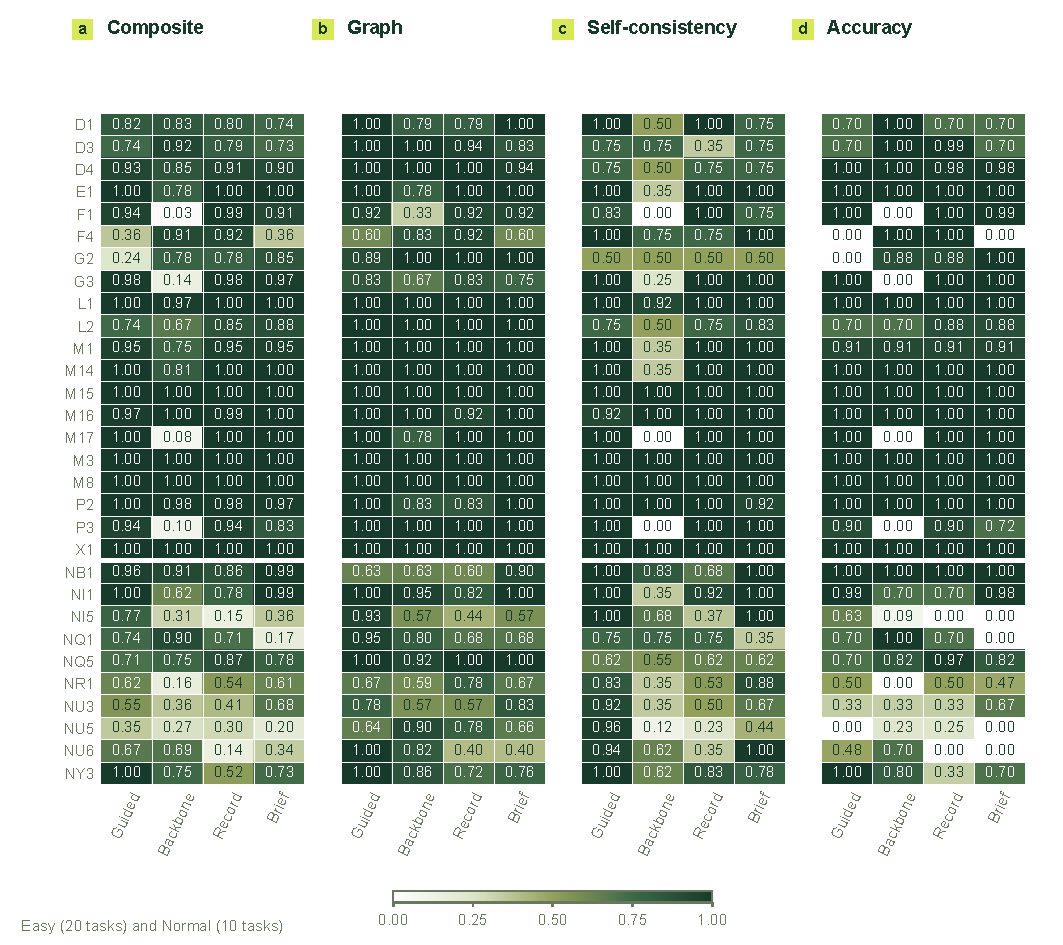
\includegraphics[width=\textwidth]{figures/bench_tasks.pdf}
\caption{All Easy and Normal task scores. Each task has four configuration rows and four score layers: composite, graph, scientific self-consistency, and accuracy. Cells are rounded to two decimals; the preceding tables and companion CSV retain greater precision. Backbone denotes Standard.}
\label{fig:si-task-matrix-en}
\end{figure}
\begin{figure}[!t]
\centering
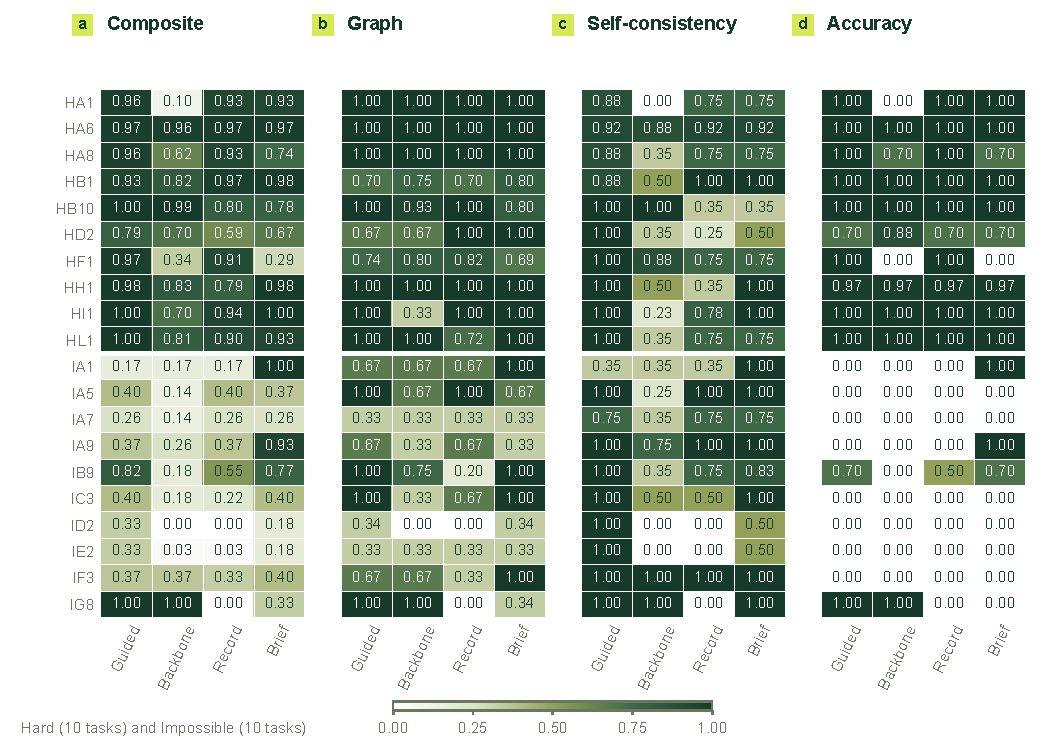
\includegraphics[width=\textwidth]{figures/bench_tasks_hi.pdf}
\caption{All Hard and Impossible task scores, with the same layer and configuration ordering as Figure~\ref{fig:si-task-matrix-en}. All 80 runs have complete composite and component values.}
\label{fig:si-task-matrix-hi}
\end{figure}

\section{Behavioral diagnostics and archived research trajectories}
\label{sec:si-behavioral}

\subsection{Study materials and local inference settings}

The behavioral studies combine archived Cloudra research trajectories with controlled local judgments about the chemical objects, measured quantities, and evidence associations appearing in those trajectories. Historical research events retain their original statements, inputs, returned artifacts, and subsequent actions. Local probes supply frozen questions derived from those events and record the model's answer under specified information and answer-order conditions. The supplementary data retain each question, expected semantic answer, actual answer, request configuration, and source identifier.

The local deployment was archived as \texttt{qwen3.8:27b}, using a GGUF Q4\_K\_M quantization with a reported parameter size of 27.3B. The deployment digest is
\begin{quote}\small\ttfamily
22130167c4c20e20c7b71454612966ca8e8171e9b3cc8ab6ce8aa6cbfec79643.
\end{quote}
The local API metadata reports a maximum model context of 262,144 tokens. The short diagnostic requests use an 8,192-token context. Temperature is 0, seed 42, top-$k$ 0, top-$p$ 1, minimum-$p$ 0, repeat penalty 1, presence penalty 0, and draft prediction count 0. The initial identity and evidence-binding probes use the archived explicit ChatML prompt rendering, an empty thinking block, thinking disabled, and a maximum of eight generated tokens; top-20 token log probabilities are retained. The native-chat controls use separate system and user messages, the deployment's native rendering, and a maximum of 1,024 generated tokens, with the thinking setting specified per request. In every choice task, the saved final answer is evaluated as an exact permitted uppercase choice letter. Semantic answer identity is recorded separately from the displayed letter.

\begin{table}[!htbp]
\centering\small
\caption{Experimental units and crossed conditions of the local diagnostic studies.}
\label{tab:si-diagnostic-design}
\begin{tabular}{p{0.24\linewidth}p{0.57\linewidth}r}
\toprule
Study & Frozen inputs and experimental factors & Calls\\
\midrule
Chemical identity & 16 pairs $\times$ 2 representations $\times$ 2 answer orders & 64\\
Distance judgment & 4 geometries $\times$ 2 information conditions $\times$ 2 answer orders $\times$ 2 thinking settings & 32\\
Target-angle feedback & 2 information conditions; 3 cyclic next-action permutations and 2 sufficiency permutations per condition & 10\\
Evidence associations & 4 chains $\times$ 2 association conditions $\times$ 2 presentations $\times$ 2 answer orders & 32\\
Native diagnostic follow-up & 20 identity inputs and 16 association inputs, each under 2 thinking settings & 72\\
Outstanding requirements & 3 state questions $\times$ 2 context conditions $\times$ 2 answer orders & 12\\
\bottomrule
\end{tabular}
\par\smallskip\begin{minipage}{\linewidth}\footnotesize
Call counts retain the actual experimental units. Equivalent representations, answer-order variants, and information conditions are paired versions of the same source object. The single expanded-budget distance follow-up is additional to the 32-call distance study. The activation replacement experiment is described separately below.
\end{minipage}
\end{table}

\subsection{Chemical identity under equivalent representations and answer reversal}

Sixteen molecular-identity pairs were derived from four task systems. They cover identical identities, same-formula connectivity changes, connectivity and formal-charge relocation, double-bond stereochemistry, and protonation changes. For each pair, the original notation and an equivalent rewriting were crossed with two answer orders. In the forward order, A means the same represented chemical identity and B means different represented chemical identities; in the swapped order these meanings exchange. The questions instruct the model to preserve connectivity, bond orders, formal charges, and specified stereochemistry while treating traversal order, ring digits, and disconnected-component order as notation.

Across the resulting 64 judgments, 58 answers were correct. At fixed identity pair and answer order, equivalent rewriting changed the semantic answer in four of 32 comparisons. At fixed pair and representation, reversing answer order changed the semantic answer in six of 32 comparisons. All six order-sensitive cases selected A in both displayed orders. The same-formula example \texttt{CC1CC=C1} versus \texttt{C=C1CCC1} places the double bond within and outside the ring, respectively. The saved model answer is A in all four representation/order conditions, although the chemical meaning of A changes with the answer order. This design isolates persistent chemical identity from a particular string traversal or preferred answer position.

The identical-string positive conditions provide a baseline for matching a representation to itself. Equivalent rewritings test whether that judgment survives a notation change. Different-identity controls ask whether molecular formula agreement can coexist with an actual change of connectivity or stereochemistry. The complete frozen strings and semantic labels are retained with the diagnostic data, allowing these contrasts to be reconstructed for every pair.

\subsection{XYZ coordinates and explicitly measured distances}

Four NB1 geometries were selected from the archived research trajectories. The local question asks which of two specified atom pairs has the shorter Euclidean distance. The original-XYZ condition supplies the complete geometry in its saved atom order. The measured-distance condition supplies program-calculated values for the same atom pairs. Each condition appears in both answer orders and in direct-answer and thinking modes, yielding 32 native chat calls. Table~\ref{tab:si-distance-stimuli} gives the measured values used to construct the paired conditions; all atom indices are one-based.

\begin{table}[!htbp]
\centering\small
\caption{Distance comparisons derived from the four archived NB1 geometries.}
\label{tab:si-distance-stimuli}
\begin{tabular}{llrlr}
\toprule
Source workflow & Pair 1 & $d_1$ (\AA) & Pair 2 & $d_2$ (\AA)\\
\midrule
Guided & C2--C4 & 2.029 & O3--H8 & 1.248\\
Brief & C4--H11 & 2.197 & O7--H11 & 0.981\\
Brief & C4--H11 & 1.388 & O7--H11 & 1.362\\
Brief & C4--H11 & 2.386 & O7--H11 & 0.968\\
\bottomrule
\end{tabular}
\end{table}

\begin{table}[!htbp]
\centering\small
\caption{Complete outcomes of the native distance-judgment controls.}
\label{tab:si-distance-outcomes}
\begin{tabular}{llrrrr}
\toprule
Thinking & Information & Calls & Correct & Valid wrong & Budget-truncated\\
\midrule
Off & XYZ coordinates & 8 & 4 & 4 & 0\\
Off & Measured distances & 8 & 8 & 0 & 0\\
On & XYZ coordinates & 8 & 7 & 0 & 1\\
On & Measured distances & 8 & 8 & 0 & 0\\
\bottomrule
\end{tabular}
\par\smallskip\begin{minipage}{\linewidth}\footnotesize
A budget-truncated generation reached the 1,024-token ceiling with no final choice. It remains in the eight-input denominator. A separate 2,048-token follow-up of that one input produced the correct choice after 1,353 generated tokens.
\end{minipage}
\end{table}

All eight direct-answer XYZ responses selected A, giving four correct answers and no semantic agreement across the four answer-reversed source pairs. Providing the measured distances gave eight correct answers in each thinking setting and preserved the semantic answer under reversal. With thinking enabled, median generated-token counts over the eight matched inputs were 807.5 for XYZ and 86 for measured distances. The archived generated-token count includes thinking tokens where enabled. Supplying the measurements makes the relevant physical relation explicit and removes its repeated numerical reconstruction from the subsequent choice. This allocation complements the use of program-executed numerical operations in program-aided language models.\citep{ref15}

\subsection{Target-specific geometric feedback in an E1 operation chain}

The E1 source trajectory specifies the transferring hydrogen H7 in the H7--C2--C3--Cl4 dihedral and seeks an anti-periplanar arrangement near $180^\circ$. Rotation of the C3-side fragment about C2--C3 by $+120^\circ$ and $-120^\circ$ produces candidates A and B, while the C3--Cl4 distance is set to 2.35 \AA. The default structural report describes a dihedral involving H5. The subsequent explicit H7 measurement identifies the quantity required by the current research objective.

\begin{table}[!htbp]
\centering\small
\caption{Dihedral measurements and circular residuals for the saved E1 candidates.}
\label{tab:si-target-dihedrals}
\begin{tabular}{llrr}
\toprule
Candidate & Atom quadruplet & Signed angle ($^\circ$) & Distance to $180^\circ$\\
\midrule
A & H5--C2--C3--Cl4 & $-55.7831$ & 124.2169\\
A & H7--C2--C3--Cl4 & 59.3752 & 120.6248\\
B & H5--C2--C3--Cl4 & 64.2169 & 115.7831\\
B & H7--C2--C3--Cl4 & 179.3752 & 0.6248\\
\bottomrule
\end{tabular}
\end{table}

The Newman projections in the manuscript are drawn from the saved candidate coordinates by projection normal to C2$\to$C3, with projected bond directions normalized for display. Table~\ref{tab:si-target-dihedrals} retains the measured signed angles and circular distances to the target. Candidate B is subsequently supplied as the transition-state guess in the actual trajectory. Its submission identifies the H7-based anti-periplanar arrangement and the stretched C3--Cl4 bond as the geometric rationale.

Ten local probes then separate the available measurement from the action question. In the H5-only condition, the H7 values and XYZ geometry are withheld. In the H5-plus-H7 condition, the measured target values are supplied. For next-action questions, all three cyclic option permutations switch from requesting the H7 measurement to selecting candidate B when the target values are added. Two paired information-sufficiency tests likewise switch from requesting additional target information to declaring the comparison sufficient. The facts used by these probes are measurements from the saved geometries. The controlled intervention is which measured quantities are supplied to the decision.

\subsection{Single-token transfer of a reported numerical fact}

The activation experiment uses the archived local quantized model for a reported-distance comparison.\citep{ref16} We changed the first reported distance from 2.029 to 1.029~\AA. The second distance remains 1.248~\AA. This reverses the correct comparison. The clean and edited prompts each contain 124 tokens; their token IDs differ only at global position 53, corresponding to the initial digit of the changed measurement. The original-fact answer is B in the forward option order and A in the reversed order.

For each option order, the residual-stream state at position 53 is captured from the original prompt and transferred into the edited prompt at zero-based layers 7, 15, 31, and 47. The four layers are fixed in the experiment manifest. The readout is the full-vocabulary softmax probability mass assigned to the original-fact answer, summing its bare-letter and leading-space spellings. Table~\ref{tab:si-fact-patch} preserves the clean, edited, and transferred-state values.

\begin{table}[!htbp]
\centering\small
\caption{Probability of the original-fact answer under single-position activation replacement.}
\label{tab:si-fact-patch}
\begin{tabular}{lrr}
\toprule
Input / intervention & Forward: original answer B & Reversed: original answer A\\
\midrule
Original input & 0.954032 & 0.996932\\
Edited input & 0.008694 & 0.073626\\
Transfer at layer 7 & 0.029099 & 0.955908\\
Transfer at layer 15 & 0.015033 & 0.717660\\
Transfer at layer 31 & 0.007961 & 0.072117\\
Transfer at layer 47 & 0.008763 & 0.069810\\
\bottomrule
\end{tabular}
\par\smallskip\begin{minipage}{\linewidth}\footnotesize
The readout uses the full vocabulary, with bare and leading-space answer tokens combined. It is distinct from an A/B-renormalized probability or a proportion of correct task runs.
\end{minipage}
\end{table}

Two controls are executed in both option orders. Self-replacement transfers the edited prompt's own state at the changed fact token; the prefix control transfers at unchanged token position 0. Both produce exactly equal full-vocabulary logits to the edited baseline, with a maximum absolute logit difference of 0. In the reversed order, layer-7 and layer-15 transfers restore substantial probability to the original-fact answer. In the forward order, the corresponding changes are smaller and the edited answer remains preferred. The result connects a localized representation of a supplied measurement to the subsequent choice while retaining the answer-order asymmetry in the numerical record.

\subsection{Evidence associations under fixed local calculation facts}

Four source evidence chains from three tasks are used to construct paired coherent and altered-association records. The two NB1 chains share one source run. Each record appears in a flat list and an explicitly linked representation, with both answer orders. This yields $4\times2\times2\times2=32$ inputs. Each altered record changes a single association: the geometry used by the saddle-frequency calculation, the IRC starting geometry, the optimization input for a terminal IRC frame, or the identity of the target species. Local normal-termination flags, convergence flags, energies, and imaginary-frequency values remain fixed.

The question asks whether the supplied associations meet the specified support requirements for the indicated reaction step. Linked presentations give the optimized saddle, frequency geometry, IRC start, terminal frames, endpoint optimization/frequency chain, and declared species as explicit references. The model answers all 16 linked inputs correctly and 14 of 16 flat inputs correctly. Both flat-presentation errors occur in altered records with reversed answer options, in E1 and the second NB1 step. The paired records show how the scientific role of a calculation changes when its association changes, even though its local numerical values are unchanged. Explicit relational encoding gives the model direct access to this organization.\citep{ref17}

A subsequent native-chat follow-up uses the two source chains implicated by these errors and retains every coherent/altered, flat/linked, and option-order variant, giving 16 association questions per thinking mode. The same follow-up also retains all four variants of five identity pairs implicated by the first-stage identity results, giving 20 identity questions per mode. Table~\ref{tab:si-native-followup} records every outcome category in this 72-call follow-up. Under native chat with thinking disabled, the selected identity and association counts remain 14/20 and 14/16 correct. With thinking enabled, association judgments reach 16/16; the identity family has eight correct final choices and 12 budget-truncated generations at the common 1,024-token maximum.

\begin{table}[!htbp]
\centering\small
\caption{Complete outcomes for the selected native diagnostic follow-up.}
\label{tab:si-native-followup}
\begin{tabular}{llrrrr}
\toprule
Rendering / mode & Family & Calls & Correct & Valid wrong & Budget-truncated\\
\midrule
First-stage raw & Identity & 20 & 14 & 6 & 0\\
First-stage raw & Association & 16 & 14 & 2 & 0\\
Native, thinking off & Identity & 20 & 14 & 6 & 0\\
Native, thinking off & Association & 16 & 14 & 2 & 0\\
Native, thinking on & Identity & 20 & 8 & 0 & 12\\
Native, thinking on & Association & 16 & 16 & 0 & 0\\
\bottomrule
\end{tabular}
\par\smallskip\begin{minipage}{\linewidth}\footnotesize
The first-stage rows are the selected records from the existing 96-input identity/association study. The four native rows contain 72 additional calls. All selected base cases retain their complete frozen variants; budget-truncated inputs remain in the denominators.
\end{minipage}
\end{table}

\subsection{From a detected gap to the next research action}

The historical HA1 and NB1 examples provide the corresponding research-level sequence. In a Brief HA1 trajectory, compact diagnostics were followed by changes to the source-minimum reference while the IRC endpoint association remained unresolved. In a Guided NB1 trajectory, a frequency result with zero imaginary modes was reported as a normal-mode defect. The Coordinator then requested changes to the transition-state guess and optimization constraints, and the subsequent calculation used the revised parameters. Each source sequence retains the diagnostic, the next scientific instruction, and the resulting computational request. This follows the relation between feedback and a concrete revision rather than using a tool-success flag as the outcome.\citep{ref18}

The IA1 completion sequence addresses another decision. Its delivery report has \texttt{complete=false}, an unresolved bidirectional short-IRC requirement, and no formal waiver. The Coordinator nevertheless requests a complete stop after earlier affirmative comments about intermediate optimization. The completion check returns the remaining IRC requirement to the active research context. The next stop request explicitly changes its disposition to partial. The sequence records the actual claim change and the outstanding path requirement.

The local state-reading study extracts three questions from this IA1 source: whether the latest report declares completion, whether a formal short-IRC waiver exists, and whether the evidence gap should remain outstanding. Each is asked in a report-only context and a quoted 12-message context, with both answer orders. All 12 judgments agree with the frozen state labels. All six option-reversed pairs retain the same semantic answer. The expected answer is derived from the explicit report fields and waiver list, providing a persistent reference for subsequent completion decisions.

\subsection{Discussion of the diagnostic scope}

These experiments resolve distinct operations in the research process: maintaining identity across representations, obtaining a spatial relation, matching feedback to the atoms named in an objective, transmitting a reported fact, connecting calculation artifacts, and reading outstanding scientific requirements. The local measurements identify where explicit representations change the model's decisions. Their interpretation is specific to the archived local deployment, frozen sources, and experimental contrasts. The native follow-up selects sources after inspection of first-stage errors, while retaining complete variants; its counts describe that selected set. Native thinking also changes conditioning and consumed generation, so a common maximum output budget does not imply matched computation.

The activation replacement establishes a local effect on a reported numerical comparison in the quantized Qwen deployment. Its readout does not identify an internal mechanism of the original DeepSeek research runs or a direct measurement of chemical validity. The E1 historical transition to candidate B is observational, with an intervening Supervisor/workspace input before the next model action. The separate local feedback probes isolate supplied target measurements under the curated comparisons.

The completed IA1 state-reading result covers the report-only and 12-message conditions. An additional full 306-message history request contained 242,803 counted input tokens in a 262,144-token context and reached the 3,600-s HTTP waiting limit without a saved answer. Only the first of six planned full-history inputs was attempted; the other five were not attempted. This execution status is retained separately from the 12 completed short-context judgments. Across the diagnostics, generated-answer accuracy, execution status, evidence-association agreement, and scientific acceptance remain distinct observations.

\section{Literature sample and source-linked capability register}
\label{sec:si-literature}
\subsection{Selection and coding procedure}
The literature sample retained 85 separately described chemical AI agent systems, architectures, or workflows in the 27 October 2026 source snapshot. Inclusion required an LLM to participate in planning, tool use, input/code modification, or feedback-driven decisions in an executed molecular, atomistic, or molecular coarse-grained physical calculation. The unit was a described system or workflow: journal/preprint versions and aliases were reconciled to the same record. The register retains the original sources, evidence locations, and descriptions used for coding.

Records were assigned according to the physical objects demonstrated in their worked examples: materials, crystals, and surfaces (39); finite molecules and complexes (23); liquids, soft matter, and biomolecules (12); or demonstrations spanning multiple object classes (11). Periodicity alone did not determine the class: a protein, liquid, or polymer simulation box remained associated with its actual physical object. Cloudra itself is shown separately in the manuscript figures and is not added to the 85-record denominator.

Task codes denote demonstrated activities: T, structure construction/editing; E, separately demonstrated static energy, electronic structure, or material-property calculations; O, geometry optimization/relaxation; F, vibrations/frequencies and associated thermochemistry; R, explicit reaction paths or transition-state searches, including solid-state NEB; D, molecular or quantum dynamics. A record can carry multiple task codes. The respective code counts are 61, 61, 53, 22, 11, and 37. Empty codes are unencoded activities in this source sample. Coarse-grained normal modes and MD-derived free-energy profiles retain their specific physical meaning in the evidence register.

\subsection{Source register and counting variants}
Table~\ref{tab:si-literature} links every system to its primary article or official project record and to additional evidence sources where applicable. The machine-readable files \path{companion_data/literature/systems.json} and \path{companion_data/literature/source_index.csv} preserve the exact source locations and supporting descriptions for each assigned code. They also retain the demonstrated targets, boundary conditions, aliases, family assignments, and access/source qualifications. A crosswalk to the 49-system review used during source discovery is supplied with the screening and search records.

The main manuscript uses separately described systems/workflows. Grouping the specified El Agente, MDAgent, MatAgent/ChatMat, and DynaMate/DynaMate2 families gives 75 records (37 materials/surfaces, 17 molecules/complexes, 11 soft/biomolecular, and 10 multiple-class records). Excluding the three official-demonstration-only systems gives 82 records (38, 21, 12, 11); additionally excluding MLP Copilot gives 81 (37, 21, 12, 11). These counting variants are retained with their definitions in the source data.

\begingroup
\small
\setlength{\tabcolsep}{3pt}
\renewcommand{\arraystretch}{1.12}
\begin{longtable}{@{}p{0.05\linewidth}p{0.35\linewidth}p{0.17\linewidth}p{0.16\linewidth}p{0.17\linewidth}@{}}
\caption{Complete source-linked register of the 85 chemical AI agent systems/workflows used in the literature sample. Task codes are defined in the text. L01--L85 link to the primary records; lettered links give additional sources.}\label{tab:si-literature}\\
\toprule
No. & System/workflow & Demonstrated object class & Task codes & Original sources \\
\midrule
\endfirsthead
\multicolumn{5}{l}{\tablename\ \thetable\ (continued)}\\
\toprule
No. & System/workflow & Demonstrated object class & Task codes & Original sources \\
\midrule
\endhead
\midrule
\multicolumn{5}{r}{Continued on the next page}\\
\endfoot
\bottomrule
\endlastfoot
1 & Buehler molecular-DFT multi-agent demonstration & Molecules/complexes & T E & \href{https://pubs.acs.org/doi/abs/10.1021/acsengineeringau.3c00058}{L01}, \href{https://arxiv.org/abs/2310.19998}{a} \\
\addlinespace[2pt]
2 & ProtAgents & Soft/biomolecular & T F & \href{https://arxiv.org/html/2402.04268v1}{L02}, \href{https://arxiv.org/abs/2402.04268}{a} \\
\addlinespace[2pt]
3 & LLaMP & Materials/surfaces & T D & \href{https://arxiv.org/html/2401.17244v3}{L03} \\
\addlinespace[2pt]
4 & ChemReasoner & Materials/surfaces & E O T & \href{https://arxiv.org/html/2402.10980v3}{L04} \\
\addlinespace[2pt]
5 & AtomAgents & Materials/surfaces & T E O R & \href{https://arxiv.org/html/2407.10022v1}{L05} \\
\addlinespace[2pt]
6 & Adsorb-Agent & Materials/surfaces & T E O & \href{https://arxiv.org/html/2410.16658v4}{L06} \\
\addlinespace[2pt]
7 & LangSim & Materials/surfaces & T E O & \href{https://arxiv.org/html/2411.15221v1}{L07}, \href{https://www.mpie.de/5063016/LangSim}{a} \\
\addlinespace[2pt]
8 & MDCrow & Soft/biomolecular & D & \href{https://arxiv.org/html/2502.09565v1}{L08} \\
\addlinespace[2pt]
9 & MDAgent & Materials/surfaces & D & \href{https://www.nature.com/articles/s41598-025-92337-6}{L09} \\
\addlinespace[2pt]
10 & El Agente Q & Molecules/complexes & T E O F & \href{https://arxiv.org/abs/2505.02484}{L10} \\
\addlinespace[2pt]
11 & Aitomia & Molecules/complexes & T E O F & \href{https://arxiv.org/pdf/2505.08195}{L11} \\
\addlinespace[2pt]
12 & DynaMate (Mendible-Barreto et al.) & Multiple classes & T O D & \href{https://pubs.rsc.org/en/content/articlehtml/2025/me/d5me00062a}{L12}, \href{https://www.researchgate.net/publication/391996468_DynaMate_leveraging_AI-agents_for_customized_research_workflows}{a}, \href{https://github.com/omendibleba/DynaMate}{b} \\
\addlinespace[2pt]
13 & MatAgent (Lv et al.) & Molecules/complexes & T E & \href{https://onlinelibrary.wiley.com/doi/full/10.1002/mgea.70013}{L13} \\
\addlinespace[2pt]
14 & ChemGraph & Molecules/complexes & T E O F & \href{https://www.nature.com/articles/s42004-025-01776-9}{L14} \\
\addlinespace[2pt]
15 & TopoMAS & Materials/surfaces & T E & \href{https://arxiv.org/html/2507.04053v1}{L15} \\
\addlinespace[2pt]
16 & NAMD-Agent & Soft/biomolecular & T D & \href{https://arxiv.org/html/2507.07887v1}{L16}, \href{https://arxiv.org/html/2507.07887v2}{a} \\
\addlinespace[2pt]
17 & DREAMS & Materials/surfaces & T E O & \href{https://arxiv.org/html/2507.14267v2}{L17} \\
\addlinespace[2pt]
18 & SparksMatter & Materials/surfaces & T E O & \href{https://arxiv.org/html/2508.02956v1}{L18} \\
\addlinespace[2pt]
19 & AutoSolvate-Agent & Molecules/complexes & T E O F & \href{https://openreview.net/pdf?id=ATEtqdGn6W}{L19}, \href{https://openreview.net/pdf/395d4c9eda83111a078ba05d86adcf84ec77e4aa.pdf}{a}, \href{https://www.linkedin.com/in/fren5}{b} \\
\addlinespace[2pt]
20 & VASPilot & Materials/surfaces & E O & \href{https://arxiv.org/abs/2508.07035}{L20} \\
\addlinespace[2pt]
21 & ChemAgents molecular simulation workflow & Molecules/complexes & F D & \href{https://pubs.rsc.org/en/content/articlehtml/2026/sc/d5sc08794e}{L21}, \href{https://doi.org/10.26434/chemrxiv-2025-4kh1r}{a} \\
\addlinespace[2pt]
22 & AMLP & Materials/surfaces & E O D & \href{https://arxiv.org/html/2509.21647v1}{L22} \\
\addlinespace[2pt]
23 & ToPolyAgent & Soft/biomolecular & T D & \href{https://arxiv.org/html/2510.12091v1}{L23}, \href{https://arxiv.org/abs/2510.12091}{a} \\
\addlinespace[2pt]
24 & GENIUS & Materials/surfaces & E O & \href{https://arxiv.org/html/2512.06404v1}{L24}, \href{https://www.nature.com/articles/s43246-026-01167-0}{a} \\
\addlinespace[2pt]
25 & LAMMPS-Agents & Materials/surfaces & T E O F D & \href{https://github.com/ANL-NST/LAMMPS-Agents}{L25}, \href{https://doi.org/10.1039/D5DD00435G}{a}, \href{https://www.alcf.anl.gov/publications/multi-agentic-ai-framework-end-end-atomistic-simulations}{b} \\
\addlinespace[2pt]
26 & DynaMate (protein--ligand) & Soft/biomolecular & T O D & \href{https://arxiv.org/html/2512.10034v1}{L26}, \href{https://openreview.net/pdf?id=NkLAjIzwei}{a} \\
\addlinespace[2pt]
27 & AGAPI-Agents & Materials/surfaces & T E O & \href{https://arxiv.org/html/2512.11935v1}{L27} \\
\addlinespace[2pt]
28 & MASTER & Materials/surfaces & T E O & \href{https://arxiv.org/html/2512.13930v1}{L28} \\
\addlinespace[2pt]
29 & El Agente Cuántico & Molecules/complexes & E & \href{https://arxiv.org/html/2512.18847v3}{L29}, \href{https://arxiv.org/abs/2512.18847}{a} \\
\addlinespace[2pt]
30 & VASP Agent & Materials/surfaces & E O R & \href{https://arxiv.org/html/2512.19458v1}{L30} \\
\addlinespace[2pt]
31 & Masgent & Materials/surfaces & T E O & \href{https://arxiv.org/pdf/2512.23010}{L31} \\
\addlinespace[2pt]
32 & CASCADE & Materials/surfaces & E O & \href{https://arxiv.org/html/2512.23880v1}{L32} \\
\addlinespace[2pt]
33 & MDAgent2-RUNTIME & Materials/surfaces & D & \href{https://arxiv.org/html/2601.02075v1}{L33}, \href{https://github.com/FredericVAN/PKU_MDAgent2}{a} \\
\addlinespace[2pt]
34 & CatMaster & Materials/surfaces & T E O F R & \href{https://arxiv.org/html/2601.13508v3}{L34} \\
\addlinespace[2pt]
35 & QUASAR & Multiple classes & T E O D & \href{https://arxiv.org/html/2602.00185v1}{L35} \\
\addlinespace[2pt]
36 & ChatMat & Molecules/complexes & T E & \href{https://www.researchgate.net/publication/404118299_ChatMat_A_Multi-Agent_Chemist_for_Autonomous_Material_Prediction_and_Exploration}{L36}, \href{https://doi.org/10.1039/D5DD00582E}{a}, \href{https://zenodo.org/records/18459314}{b}, \href{https://github.com/Xiaobu-USTC/ChatMat}{c} \\
\addlinespace[2pt]
37 & El Agente Estructural & Molecules/complexes & T O & \href{https://arxiv.org/html/2602.04849v1}{L37} \\
\addlinespace[2pt]
38 & El Agente Quntur & Molecules/complexes & T E O F R & \href{https://arxiv.org/html/2602.04850v3}{L38} \\
\addlinespace[2pt]
39 & El Agente Gráfico & Multiple classes & T E O F & \href{https://arxiv.org/html/2602.17902v1}{L39}, \href{https://arxiv.org/html/2602.17902v2}{a} \\
\addlinespace[2pt]
40 & El Agente Sólido & Materials/surfaces & T E O F & \href{https://arxiv.org/html/2602.17886v1}{L40} \\
\addlinespace[2pt]
41 & Catalyst-Agent & Materials/surfaces & T E O & \href{https://arxiv.org/html/2603.01311v1}{L41} \\
\addlinespace[2pt]
42 & TritonDFT & Materials/surfaces & E O F & \href{https://arxiv.org/html/2603.03372v1}{L42} \\
\addlinespace[2pt]
43 & Chelatron & Molecules/complexes & T E & \href{https://science.osti.gov/-/media/About/pdf/scac/meetings/2026/lab-contributions-to-GM-03-24-2026v2.pdf}{L43} \\
\addlinespace[2pt]
44 & Electrolyte Agent / Reasoning-to-Simulation & Soft/biomolecular & T D & \href{https://openreview.net/pdf/837f62f17b0f4210dbc1260e813b7fd1ebabd467.pdf}{L44}, \href{https://zenodo.org/records/19198509}{a} \\
\addlinespace[2pt]
45 & MatSciAgent & Materials/surfaces & T D & \href{https://www.nature.com/articles/s43246-025-00994-x}{L45} \\
\addlinespace[2pt]
46 & OpenClaw computational-chemistry skills workflow & Molecules/complexes & T O D & \href{https://arxiv.org/html/2603.25522v1}{L46} \\
\addlinespace[2pt]
47 & Protomia & Molecules/complexes & T E F & \href{https://aitomistic.com/protomia/docs/research-workflow}{L47}, \href{https://arxiv.org/html/2608.18508v1}{a} \\
\addlinespace[2pt]
48 & SimMOF & Materials/surfaces & T E O D & \href{https://arxiv.org/pdf/2603.29152}{L48} \\
\addlinespace[2pt]
49 & PolyJarvis & Soft/biomolecular & T D & \href{https://arxiv.org/html/2604.02537v3}{L49} \\
\addlinespace[2pt]
50 & FermiLink & Multiple classes & E D & \href{https://arxiv.org/html/2604.03460v1}{L50} \\
\addlinespace[2pt]
51 & MatClaw & Materials/surfaces & E D & \href{https://arxiv.org/html/2604.02688v1}{L51} \\
\addlinespace[2pt]
52 & El Agente Forjador & Molecules/complexes & T E O F D & \href{https://arxiv.org/html/2604.14609v1}{L52} \\
\addlinespace[2pt]
53 & MDAgent (biomolecular, 2026) & Soft/biomolecular & T O D & \href{https://arxiv.org/pdf/2604.18622}{L53}, \href{https://arxiv.org/abs/2604.18622}{a} \\
\addlinespace[2pt]
54 & VirtualLab\_CC & Molecules/complexes & T E O F & \href{https://www.sciencedirect.com/science/article/pii/S2949747726000230}{L54}, \href{https://github.com/CCBG-Lab/VirtualLab_CC}{a}, \href{https://doi.org/10.26434/chemrxiv.15002407/v1}{b} \\
\addlinespace[2pt]
55 & XDFT & Materials/surfaces & T E & \href{https://arxiv.org/pdf/2604.26703v1}{L55} \\
\addlinespace[2pt]
56 & CatGo & Multiple classes & T E O F R & \href{https://www.researchgate.net/publication/410982627_CatGo_Bridging_CLI_coding_agents_with_interactive_structure_and_workflow_management_for_computational_chemistry}{L56}, \href{https://doi.org/10.1039/D6DD00273K}{a}, \href{https://zenodo.org/records/21552845}{b}, \href{https://doi.org/10.26434/chemrxiv.15002984/v1}{c} \\
\addlinespace[2pt]
57 & TSAgent & Materials/surfaces & E O F R & \href{https://arxiv.org/html/2605.14154v1}{L57} \\
\addlinespace[2pt]
58 & Lang2MLIP & Materials/surfaces & T E D & \href{https://arxiv.org/html/2605.14527v1}{L58} \\
\addlinespace[2pt]
59 & AtomisticSkills & Multiple classes & T E O D & \href{https://arxiv.org/html/2605.24002v1}{L59} \\
\addlinespace[2pt]
60 & DynaMate2 & Soft/biomolecular & T D & \href{https://arxiv.org/pdf/2605.20819v2}{L60}, \href{https://arxiv.org/abs/2605.20819}{a} \\
\addlinespace[2pt]
61 & ChatMOSP & Materials/surfaces & T & \href{https://arxiv.org/pdf/2605.24265}{L61} \\
\addlinespace[2pt]
62 & AutoDFT & Multiple classes & E O F D & \href{https://arxiv.org/html/2605.26179v1}{L62} \\
\addlinespace[2pt]
63 & MLIPilot & Multiple classes & E O D & \href{https://arxiv.org/html/2605.30889v1}{L63} \\
\addlinespace[2pt]
64 & CatDT & Materials/surfaces & T E O F R & \href{https://arxiv.org/html/2606.05050v2}{L64} \\
\addlinespace[2pt]
65 & Paimon & Multiple classes & T O D & \href{https://arxiv.org/html/2606.09422v1}{L65} \\
\addlinespace[2pt]
66 & MDForge & Soft/biomolecular & D & \href{https://arxiv.org/html/2606.12916v2}{L66} \\
\addlinespace[2pt]
67 & URSA LAMMPS agent & Materials/surfaces & T E D & \href{https://arxiv.org/html/2607.22596v1}{L67}, \href{https://arxiv.org/abs/2607.22596}{a} \\
\addlinespace[2pt]
68 & AdsMind & Materials/surfaces & T E O & \href{https://arxiv.org/html/2606.19152v1}{L68} \\
\addlinespace[2pt]
69 & LADeQ & Molecules/complexes & E & \href{https://arxiv.org/html/2606.20729v1}{L69} \\
\addlinespace[2pt]
70 & MutexaGPT & Soft/biomolecular & T D & \href{https://pmc.ncbi.nlm.nih.gov/articles/PMC13308407/}{L70}, \href{https://doi.org/10.1038/s43588-026-01049-y}{a} \\
\addlinespace[2pt]
71 & Agent-MD & Materials/surfaces & D & \href{https://arxiv.org/html/2608.07637v1}{L71} \\
\addlinespace[2pt]
72 & CGMas & Soft/biomolecular & T O D & \href{https://arxiv.org/html/2608.06694v1}{L72} \\
\addlinespace[2pt]
73 & matmcp & Materials/surfaces & T E O & \href{https://github.com/Crystalhihihi/matmcp}{L73}, \href{https://raw.githubusercontent.com/Crystalhihihi/matmcp/main/docs/experiments.md}{a}, \href{https://github.com/Crystalhihihi/matmcp/tree/main/evidence/20261009-225541_mos2_d84a}{b} \\
\addlinespace[2pt]
74 & Evolving TS workflows & Molecules/complexes & O F R & \href{https://www.nature.com/articles/s41524-026-02301-9}{L74} \\
\addlinespace[2pt]
75 & ARCHE & Molecules/complexes & T E O F R & \href{https://arxiv.org/abs/2609.11147}{L75} \\
\addlinespace[2pt]
76 & Multireference QC agent & Molecules/complexes & E & \href{https://arxiv.org/html/2609.13357v1}{L76} \\
\addlinespace[2pt]
77 & El Agente Potente & Multiple classes & T E O F R D & \href{https://arxiv.org/html/2609.14840v1}{L77} \\
\addlinespace[2pt]
78 & PVmatAgent & Materials/surfaces & T E O & \href{https://onlinelibrary.wiley.com/doi/10.1002/mgea.70102}{L78}, \href{https://github.com/Albertdeng23/PVMatAgent}{a}, \href{https://doi.org/10.26434/chemrxiv.15003915/v1}{b} \\
\addlinespace[2pt]
79 & Agent-E2MD & Materials/surfaces & E O D & \href{https://arxiv.org/html/2609.26657v1}{L79} \\
\addlinespace[2pt]
80 & SQD-Agent & Molecules/complexes & E & \href{https://arxiv.org/html/2609.39302v1}{L80} \\
\addlinespace[2pt]
81 & QAOS / Quantum Agentic Operating System & Molecules/complexes & T E O & \href{https://arxiv.org/html/2610.05304v1}{L81}, \href{https://arxiv.org/abs/2610.05304}{a} \\
\addlinespace[2pt]
82 & MLP Copilot & Materials/surfaces & E D & \href{https://pmc.ncbi.nlm.nih.gov/articles/PMC13684298/}{L82}, \href{https://github.com/flarecentury/mlpcopilot}{a} \\
\addlinespace[2pt]
83 & Magnolia & Multiple classes & T E O D & \href{https://arxiv.org/html/2610.27230v1}{L83} \\
\addlinespace[2pt]
84 & GBClaw & Materials/surfaces & T E O R & \href{https://arxiv.org/pdf/2610.28629}{L84}, \href{https://zhugroup.gatech.edu/gbclaw-demo}{a} \\
\addlinespace[2pt]
85 & PULSES & Molecules/complexes & T E O D & \href{https://arxiv.org/pdf/2610.32392}{L85}, \href{https://arxiv.org/abs/2610.32392}{a} \\
\addlinespace[2pt]
\end{longtable}
\endgroup


\section{Data, software, and reproduction materials}
\label{sec:si-reproduction}
\subsection{Public data availability}
The study data are publicly available with read-only access at \url{https://drive.google.com/drive/folders/1yZo3eJuCUuAgedQztgCtLyJcc8MZipf7}. This directory provides the full P2 campaign archive \path{Cloudra-P2-final-20261031-FULL.tar.gz}, the 48-run P1b repeated-task archive and its offline-organization supplements, the Gold reference-calculation evidence snapshot, and the compact SI companion-data archive \path{Cloudra_SI_Data.zip}. The package versions, inventories, and checksums are provided with the downloads.

The P2 archive retains the campaign records underlying the 200-run full-benchmark study. The P1b archive contains the separate 48-run repeated-task study. The Gold archive contains the reference calculation inputs, native outputs, geometries, Hessians, and associated curation records. The SI companion archive contains the task definitions, full-precision score tables, behavioral records, and publication-reproduction materials described below.

The separate \href{https://drive.google.com/drive/folders/1Zkn6_2aDlloAe-bmfd7w27zxmQKj5L9K}{complete behavioral-source archive (20261030)} provides frozen inputs and responses, activation states and logits, readable event traces, source databases and calculation records, analysis scripts, and vector figures. Its topic index and manuscript-context files retain the version-specific section and figure references.

\subsection{Machine-readable task and score records}
The supplementary source package contains \path{companion_data/cloudrabench_50_task_catalogue.csv}, the 50 formal task JSON files in \path{companion_data/task_definitions/}, and \path{companion_data/cloudrabench_200_run_scores.csv}. The task JSON files preserve the molecular inputs, task text, permitted methods, Gold graphs, and scoring settings. The score table retains full source precision for all 200 composites and all 600 components. A provenance manifest records file hashes and the displayed precision used by the printed tables.

The P2 publication-source package retains the recorded component sources, paired summaries, Brief/Impossible analyses, timing extractions, and field-level provenance used by the manuscript figures. The reproducible organization script assembles the 200-run publication table from these retained records; figure scripts derive their panels from the corresponding tables. This reproduction does not launch new electronic-structure or agent calculations.

\subsection{Software responsibilities and calculation records}
Cloudra revision 70daa5a identifies the implementation described in the main-text methods.\citep{ref14} RDKit and ETKDG supply molecular representations and coordinate embedding; MMFF94 supplies force-field relaxation.\citep{ref12,etkdg2020,ref13,mmff941996} NumPy supplies numerical array/linear-algebra operations, NetworkX supplies graph representation and matching, and cclib works with engine-specific readers to extract quantum-chemical quantities.\citep{numpy2020,networkx2008,cclib2008} ASE supplies the NEB/MDMin implementation used in standard IDPP, and Adam is used in the lightweight interpolation path.\citep{ref08,neb2000,ase2017,adam2015} Task-name semantic projections use BGE-M3 embeddings and scikit-learn PCA.\citep{bgem32024,sklearn2011} Publication tables are assembled with pandas, and the quantitative figures are drawn with Matplotlib.\citep{pandas2010,matplotlib2007}

Run-specific records identify the actual engine, model/API name, charge, spin, method, basis, and keywords used in the applicable calculation or request. Dependency lower bounds in the software distribution are installation requirements; they are not substituted for archived experiment versions. Native calculation outputs retain stationary-point energies, frequencies, normal modes, IRC geometries, and endpoint optimization/frequency lineage. The numerical barrier convention is the electronic-energy difference in Equation~\ref{eq:si-barrier}.

\subsection{Reproduction entry points}
Within the accompanying Cloudra repository, the following commands reconstruct the retained P2 publication tables and figures:
\begin{quote}\small\ttfamily
python scripts/benchmark\_p2/prepare\_publication\_data.py\\
python scripts/benchmark\_p2/plot\_benchmark\_results.py\\
python scripts/benchmark\_p2/plot\_speed\_delivery.py\\
python scripts/benchmark\_p2/plot\_imp.py
\end{quote}
The companion-data archive preserves the publication reproduction tree under \path{companion_data/publication_reproduction/}; running the four commands from that directory retains the same relative file layout. The independent timing extractions and frozen behavioral requests/responses are included. The activation archive includes the original prompts, intervention commands, captured states, and full-vocabulary logits, allowing the reported probability readouts and control equalities to be reconstructed without new model inference. Scripts for replay and analysis are retained under \path{companion_data/behavioral_scripts/}. No model weights are included. The literature directory retains the complete register, screening records, and search history used for the manuscript sample. Editable TeX files, vector figures, and the bibliography are included with this SI so that scientific content, printed values, and source records remain connected during subsequent revision.

\subsection{Data-package inventory}
The \href{https://drive.google.com/file/d/1rxeg3nLczQyiO6ZackLq-LeTxzcsxHrL/view}{SI companion-data archive} is distributed separately from the compact Overleaf typesetting project. Unpack \path{Cloudra_SI_Data.zip} beside the SI source to obtain the referenced \path{companion_data/} directory. Its subdirectories contain the following materials:
\begin{itemize}[nosep,leftmargin=1.5em]
\item \path{task_definitions/}: all 50 original task definitions, including molecular inputs and rubrics.
\item \path{publication_reproduction/}: publication input records, field provenance, bootstrap summaries, timing records, and table/figure scripts.
\item \path{behavioral/}: frozen input sets, actual request/response records, deployment snapshots, geometric/evidence source cases, and activation readouts.
\item \path{behavioral_scripts/}: the corresponding intervention and diagnostic code.
\item \path{revision_20261031/}: deployment/version metadata, archive-relative configuration and request summaries, inspected Easy-task trajectories, and the conditional Impossible target-assignment scenarios.
\item \path{literature/}: all 85 source-linked systems and the coding/search records.
\end{itemize}
A file-level SHA-256 inventory accompanies the archive. Source data are retained at their recorded precision; the SI introduces no new agent or quantum-chemical calculations.

\bibliographystyle{unsrtnat}
\bibliography{references}
\end{document}
